
\documentclass[master]{thesis-uestc}
\usepackage{listings}  % 引入 listings 宏包,用于显示代码
\title{面向长尾分布数据的自监督预训练故障诊断方法研究}{}

\author{王本浩}{Wang Benhao}
\advisor{周雪\chinesespace 教授}{Dr. Xue Zhou}
\school{电子科技大学(深圳)高等研究院}{Shenzhen Institute for Advanced Study}
\major{电子信息}{Electronic and Information Engineering}
\studentnumber{202222280517}

\begin{document}

\makecover

\begin{chineseabstract}
为了适应日益增长的宽带信号和非线性系统的工程应用,用于分析瞬态电磁散射问题的时域积分方程方法研究日趋活跃。本文以时域积分方程时间步进算法及其快速算法为研究课题,重点研究了时间步进算法的数值实现技术、后时稳定性问题以及两层平面波算法加速计算等,主要研究内容分为四部分。

……

\chinesekeyword{时域电磁散射,时域积分方程,时间步进算法,后时不稳定性,时域平面波算法}
\end{chineseabstract}

\begin{englishabstract}
With the widespread engineering applications ranging from broadband signals and non-linear systems, time-domain integral equations (TDIE) methods for analyzing transient electromagnetic scattering problems are becoming widely used nowadays. TDIE-based marching-on-in-time (MOT) scheme and its fast algorithm are researched in this dissertation, including the numerical techniques of MOT scheme, late-time stability of MOT scheme, and two-level PWTD-enhanced MOT scheme. The contents are divided into four parts shown as follows.

\englishkeyword{Time-domain Electromagnetic Scattering, Time-domain Integral Equation, Marching-on In-time (MOT) Scheme, Late-time Instability, Plane Wave Time-domain (PWTD) Algorithm}
\end{englishabstract}

\thesistableofcontents

\chapter{绪\hspace{6pt}论}

\section{研究工作的背景与意义}
旋转机械作为现代工业中的关键机械设备,长期运行在高温、疲劳、重载的复杂环境中。产生的故障可能会造成严重的事故,造成巨大的经济损失和人员伤亡。智能诊断是预测健康管理(PHM)的关键组成部分,PHM是直升机、航空发动机、风力涡轮机、高速列车等各种旋转机械中最重要的系统之一,旨在有效检测故障。传统的智能诊断方法主要包括使用信号处理方法进行特征提取和使用机器学习方法进行故障分类,这些方法已经取得了相当大的进展。然而,面对异构海量数据,由专家设计和选择的特征提取方法和从信号到条件的映射能力在很大程度上取决于先验知识,既费时又需要经验。因此,如何更精确、更有效地进行诊断仍然是一个具有挑战性的问题。

现实生活中的故障检测数据通常服从长尾分布\citing{nanjing2023faultdetection}长尾分布数据是一种偏态分布,即头部类包含了大部分正常数据,相反地,尾部类包含的故障数据量比较少。用长尾数据训练神经网络时,神经网络的性能易被头部类影响而在尾部类上表现较差,对尾部类样本的错分往往会带来更大的损失,对尾部类样本的研究更具有价值意义。因此如何基于长尾分布的故障检测数据训练故障检测模型是一个具有现实意义的难点问题\citing{cumm2023faultdiagnosis}。目前,在视觉识别长尾学习领域有诸多前沿的长尾学习方法,如变分自编码器\citing{kingma2013auto}、生成对抗网络\citing{goodfellow2020generative}、CB(Class-Balanced) Loss\citing{cui2019class}、自监督学习\citing{yang2020rethinking}、MARC决策面调整算法\citing{wang2023margin},而在故障诊断长尾学习领域常见的方案为半监督学习方法\citing{nanjing2023faultdetection}、集成学习\citing{吴亮2023基于多级学习的长尾分布下交通多目标检测}、样本加权\citing{cumm2023faultdiagnosis},少有前者应用前沿的长尾学习方法在故障诊断长尾学习领域。因此,基于前沿的长尾学习方法提出一个适用于故障诊断领域的长尾学习模型是一个具有现实意义的挑战。

目前,大部分神经网络的训练仍然使用的是有监督范式,需要耗费大量的标注数据,标注这些数据是非常耗时费力的。而自监督的提出就是为了打破对人工标注的依赖,即使在没有标注数据的情况下,也可以高效地训练网络。不同于传统的非监督学习,自监督学习通过人工构造输入数据的代理标签,然后依赖于代理标签设计神经网络的监督训练任务。神经网络从而学习到特征表示。文献\cite{zhang2021federated}指出额外的自监督预训练能够使常规的长尾学习算法获得更高的性能,且验证了自监督预训练在CIFAR-LT、ImageNet-LT等视觉识别长尾数据集上的性能提升。目前,在故障诊断长尾学习领域常见的方案为半监督学习方法、集成学习、样本加权,而少有前者应用前沿自监督预训练方法在故障诊断长尾学习领域。因此,基于自监督预训练的长尾数据故障诊断是一个具有现实意义的挑战。

\section{长尾学习方法的国内外研究历史与现状}
\subsection{长尾学习的发展历程和研究现状}
国内外处理长尾问题通常从三个方面入手。一、样本层面,减少样本数量的欠采样如随机欠采样、NearMiss\citing{shen2016near}、ENN\citing{wilson1972asymptotic};增加样本数量的过采样,如随机过采样、SMOTE\citing{chawla2002smote}、变分自编码器\citing{kingma2013auto}、生成对抗网络\citing{goodfellow2020generative}。二、损失函数层面,使用类平衡的损失函数如以数据频率的逆加权\citing{huang2016learning},OHEM(Online Hard Example Mining),Focal Loss\citing{lin2017focal}以及最新的CB(Class-Balanced) Loss\citing{cui2019class}。三、模型层面,如重复组合少数类样本与抽样的同样数量的多数类样本进行集成学习、半监督和自监督学习\citing{yang2020rethinking}、MARC决策面调整算法\citing{wang2023margin}。

目前,基于长尾分布问题,国内外做出了许多研究。例如:Liu J等人\citing{liu2020deep},介绍了一种基于特征云的数据增强手段,从方差较大的数据分布宽广的头部类中学习到类内多样性并转移到尾部类,并应用于人脸识别。Yang Y等人\citing{yang2020rethinking},介绍了不平衡样本的标签在模型训练中的价值,并提出了用半监督的学习方法使用原模型识别无标签的数据,并以获得伪标签的数据扩充原数据集,同时证明了自监督的模型预训练的有效性,且样本维度越高对性能提升越有效。吴磊等人\citing{wu2023personalized}提出了提出一种面向长尾图像的个性化专家识别算法。该算法在残差网络的基础上构建多专家学习网络,并加入个性化学习模块、信息融合模块与个性化信息增强模块,以两阶段的学习方式提升长尾图像整体的识别准确率与中、尾部类别的识别效果。吴亮等人\citing{吴亮2023基于多级学习的长尾分布下交通多目标检测}构建了多级分组分类器,提升尾部类性能的同时,避免头部类性能损失。然后设计了基于多头注意力机制的分组特征重融合模块,为多级分类器输入更精细的特征。最后,基于多级分类器提出了 Logit 联合调整的方法,以缓解组间的不平衡。Wang Y等人\citing{wang2023margin}介绍了一种对长尾视觉识别学习有效的MARC决策面调整算法,对原模型输出的预测分数额外做一次训练——只用三行代码。Cui Y等人\citing{cui2019class},介绍了CB(Class-Balanced)损失函数,在原损失函数上乘以与“独特”样本数量有关的因子从而缓解类别不平衡。CB因子与超参数β有关,平滑了由1到最常见的不平衡因子1∕n。综上,文献\cite{yang2020rethinking}为自监督预训练模型应用在故障诊断长尾学习领域提供了良好的启示,但半监督学习方法在现实的长尾学习模型可能不适用。文献\cite{wu2023personalized,吴亮2023基于多级学习的长尾分布下交通多目标检测}介绍的集成学习方法削弱样本不平衡效应是常规方法,但单个模型在训练时若融合自监督预训练的方法,性能可能会得到提升。文献\cite{wang2023margin}介绍的决策面调整算法对一般的长尾学习模型都适用,但在故障诊断模型上是否可行有待商榷,且该算法对模型性能提升的理论性解释有待完善。文献\cite{cui2019class}介绍的损失函数有着新颖的思路,但超参数β需要人工选择在应用上可能存在难点。以上大部分为学者在视觉长尾学习领域的研究,此类算法在CIFAR-LT、ImageNet-LT等视觉识别数据集取得了较好的效果,而故障诊断长尾学习领域少有前沿的长尾学习算法的应用。因此,前沿的长尾学习算法在故障诊断长尾学习领域的应用具有很高的研究价值。

\subsection{自监督预训练的发展历程和研究现状}

2019 年,MoCo\citing{He_2020_CVPR} 的提出掀起了视觉自监督学习的热潮,随后 SimCLR\citing{chen2020simple}、BYOL\citing{grill2020bootstrap}、SwAV\citing{caron2020unsupervised} 等主流自监督学习算法相继问世,使该领域呈现出百花齐放、百家争鸣的繁荣景象。2021 年末,MAE\citing{he2022masked} 的提出进一步推动了自监督学习的发展,使其达到了一个前所未有的新高度。然而,在这背后,自监督学习经历了长期的迭代与发展。

目前,国内外学者针对自监督预训练开展了大量研究。例如,在计算机视觉领域,Yang 等人\citing{yang2020rethinking} 研究了不平衡样本的标签信息在模型训练中的价值,并提出了一种半监督学习方法,该方法利用原模型识别无标签数据并生成伪标签,从而扩充原始数据集,并验证了自监督预训练的有效性。此外,该研究发现,样本维度越高,性能提升越显著,这为自监督预训练在故障诊断长尾学习领域的应用提供了有力支持。Doersch 等人\citing{doersch2015unsupervised} 提出了基于局部图像块位置预测的自监督任务,即随机抽取图像中的两个块,并训练模型预测一个块相对于另一个块的位置。Zhang 等人\citing{zhang2016colorful} 构建了基于图像上色的自监督任务,将图像转换至 CIE Lab 颜色空间,并利用 L 通道作为输入,让模型预测 a 和 b 通道的颜色信息。Gidaris 等人\citing{gidaris2018unsupervised} 通过人为旋转图像不同角度,并将旋转角度作为监督信号训练模型,以此实现图像语义特征的自监督学习。

近年来,自监督预训练方法也逐步应用于故障诊断领域,并受到广泛关注。例如,Zhang 等人\citing{zhang2022prior} 提出了基于先验知识的自监督任务,并利用卷积自编码器进行训练,在小样本学习任务上取得了良好表现。Senanayaka 等人\citing{senanayaka2020toward} 采用 One-Class SVM 输出的标签作为代理标签,并使用自监督预训练的卷积神经网络进行故障特征提取。W. Zhang 等人\citing{zhang2021federated} 提出了一种基于信号块交换的自监督任务,即通过打乱时域信号块顺序构造“伪数据”,并训练模型区分原始数据和伪数据。实验结果表明,该方法在特征提取任务中表现优异。

综上,尽管\citing{doersch2015unsupervised,zhang2016colorful,gidaris2018unsupervised} 等研究在计算机视觉领域取得了重要进展,但其方法在故障诊断任务中的直接应用仍存在一定困难。然而,这些研究的思路可为故障诊断领域的自监督预训练任务设计提供启示。例如,\citing{senanayaka2020toward} 提出的 One-Class SVM 生成的标签可结合聚类算法,使其适用于多分类任务;\citing{zhang2021federated} 提出的信号块交换方法与\citing{doersch2015unsupervised} 提出的图像块位置预测任务在思路上具有一定相似性,可探索其结合方式。此外,\citing{zhang2022prior,senanayaka2020toward,zhang2021federated} 提出的自监督预训练方法在任务设计上仍存在较大创新空间,且在长尾学习任务中的应用尚不充分。因此,故障诊断领域的自监督预训练仍处于发展初期,借鉴计算机视觉领域的前沿自监督任务,在现有基础上提出更具创新性、更高性能的自监督预训练任务,仍具有重要的研究价值和挑战。

\subsection{对比自监督学习的发展与孪生网络的应用}

自监督学习的核心目标是在无人工标注的情况下自动提取有效特征\citing{min2021cross}。近年来,对比自监督学习(contrastive self-supervised learning)作为无监督学习的一个重要分支,逐渐成为研究热点,并在图像识别任务中取得了最先进的(SOTA)性能。许多相关算法相继被提出,例如动量对比学习(Momentum Contrast, MoCo)\citing{He_2020_CVPR}、对比预测编码(Contrastive Predictive Coding, CPC)\citing{oord2018representation} 以及用于视觉表征学习的简单对比学习框架(SimCLR)\citing{chen2020simple}。

这些方法的核心思想是通过拉近相同样本的不同视图(正样本对)并推远不同样本(负样本对)来学习有意义的特征表示。这类对比学习方法通常依赖存储在记忆库(memory bank)中的大量负样本,以提高对比学习效果\citing{wu2018unsupervised}。此外,一些其他对比学习方法不依赖负样本,而是计算两个正样本对之间的相似性,例如 SwAV(Swapping Assignments between multiple Views)\citing{caron2020unsupervised}、BYOL(Bootstrap Your Own Latent)\citing{grill2020bootstrap} 以及 SDCT(Self-supervised Deep Correlation Tracking)\citing{yuan2020self}。

在对比自监督学习中,孪生网络(Siamese Network)因其适用于比较不同样本的网络结构,具有独特优势。Laine 和 Aila\citing{laine2016temporal} 提出了基于孪生网络的 $\pi$-model,用于训练深度神经网络,该方法在半监督学习场景下依赖不同的正则化规则与数据增强策略。Zheng 和 Yang\citing{zheng2019unsupervised} 提出了一种“记忆正则化”机制,其核心思想是让主模型自身(而非外部模块)学习域内知识,以实现无监督场景自适应。Zhao 等人\citing{zhao2021deep} 提出了基于相互学习(mutual learning)和知识蒸馏(knowledge distillation)的训练方法,以提高视觉目标跟踪任务的性能。

上述研究均在各自领域中引入孪生网络的思想,以解决特定问题。本文受到 SimSiam\citing{chen2021exploring} 的启发,SimSiam 采用简化的孪生网络结构,并在计算机视觉(CV)任务中展现出卓越性能。基于此,我们提出了一种新颖的轴承故障诊断框架,该框架可适用于由不同神经网络层构建的多种模型。

与其他主流方法相比,SimSiam 具有以下三大优势:
\begin{enumerate}
    \item 无需构造负样本对;
    \item 无需采用大批量训练;
    \item 无需使用动量编码器(momentum encoder)。
\end{enumerate}


\section{本文的主要贡献与创新}
本论文以时域积分方程时间步进算法的数值实现技术、后时稳定性问题以及两层平面波加速算法为重点研究内容,主要创新点与贡献如下:

\section{本论文的结构安排}
本文的章节结构安排如下:

\chapter{长尾学习及相关方法的理论基础与轴承故障数据集}
\section{长尾学习相关理论}
不平衡数据在现实世界中无处不在,大规模数据集通常表现为长尾分布。长尾分布的学习亦是故障诊断领域中常见挑战,例如正常工作状态多,故障工作状态少,或是常见故障状态和罕见故障状态的样本个数差异。现实生活中的故障检测数据通常服从长尾分布,长尾分布数据是一种偏态分布,如图\ref{fig_long_tail}所示,在现实生活中,大规模的训练样本呈现典型的长尾分布,即头部类别的样本个数较多,而尾部类别的样本个数较少,样本个数逐渐降低的分布。用长尾数据训练神经网络时,神经网络的性能易被头部类影响而在尾部类上表现较差,对尾部类样本的错分往往会带来更大的损失,对尾部类样本的研究更具有价值意义。因此如何基于长尾分布的故障检测数据训练故障检测模型是一个具有现实意义的难点问题。
\begin{figure}[h]
    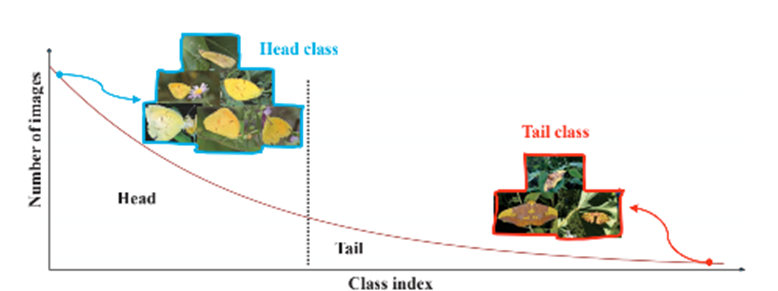
\includegraphics[width=10cm]{long_tail.png}
    \caption{长尾分布示意图}
    \label{fig_long_tail}
\end{figure}

长尾分布的样本具有非常显著的样本不均衡问题,导致训练好的模型易偏向于头部类,从而损害了对尾部类的识别效果。如图\ref{tsne_mean_distribution}所示,样本个数均衡时,各个类别之间具有清晰的区分边界,各类都占据了宽广的特征空间。而当某些类的样本个数减少呈现样本分布失衡的长尾分布时,如图\ref{tsne_lt_distribution}所示,尾部类在特征空间的分布十分狭窄,并依附在头部类附近,从而扭曲了特征空间,损害了类间的多样性和区分性。
这对现代深度学习框架提出了一个重大挑战,即使使用数据重采样方法或类平衡损失等专门技术,在极端类不平衡的情况下,仍然会出现显著的性能下降。因此,为了进一步应对这一挑战,了解类不平衡学习所带来的不同特征至关重要。然而,与平衡数据不同的是,不平衡学习背景下的标签扮演着令人惊讶的有争议的角色,这导致了标签价值的持续困境:一方面,有标签监督的学习算法通常比无监督的学习算法产生更准确的分类器,这表明了标签的积极价值;然而,另一方面,不平衡的标签在学习过程中自然会产生“标签偏差”,其中大多数类别可以显著地驱动决策边界,表明标签的负面影响。因此,不平衡的标签似乎是一把双刃剑。
\begin{figure}[h]
    \subfloat[]{
        \label{tsne_mean_distribution}
        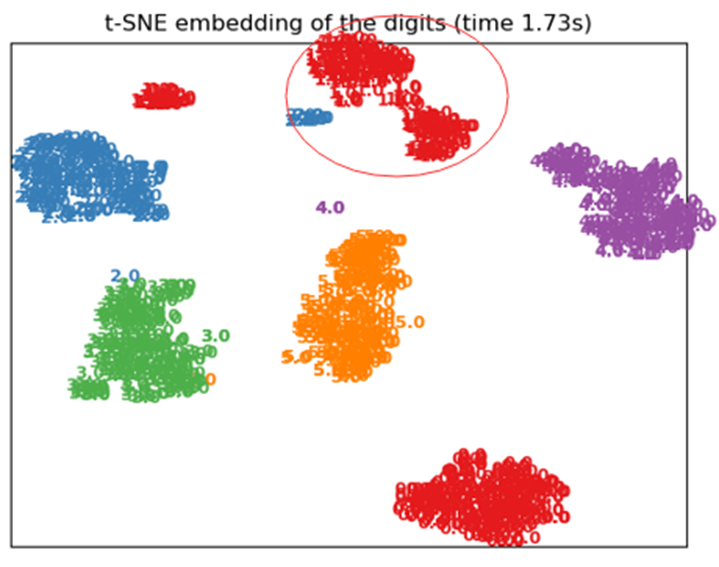
\includegraphics[width=6.77cm]{tsne_mean_distribution.png}
    }
    \subfloat[]{
        \label{tsne_lt_distribution}
        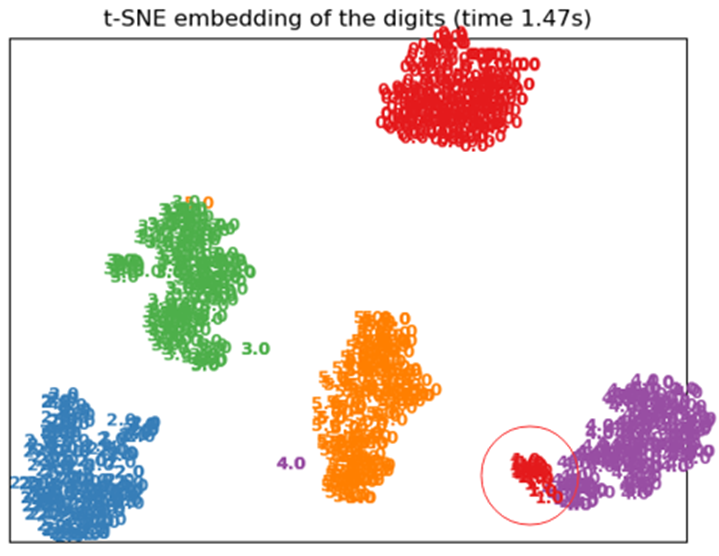
\includegraphics[width=6.77cm]{tsne_lt_distribution.png}
    }
    \caption{均匀/长尾分布数据的tsne图(a)样本均匀分布时的T-SNE分布图;(b)尾部类“1”类样本个为30,头部类样本个数为180个时的T-SNE分布图}
    \label{long-tail result}
\end{figure}

\section{自监督学习相关理论}
自监督学习是一种范式,利用“代理任务”(pretext)从大规模的无标签数据本身的内在结构挖掘通用的表征信息,通过这种构造的监督信息对网络进行训练,从而可以学习到对下游任务有价值的表征。如图\ref{self_supervise_procedure}所示,自监督学习分为两个阶段:(1)自监督预训练阶段。完全放弃标签信息,专注于数据本身,通过自监督学习进行预训练。从不平衡数据中学习标签不可知的特征表示,减少类别偏差对初始化的影响。(2)微调阶段。使用第一阶段中通过自监督预训练的网络权重作为初始化。在此基础上,可以使用任何标准的不平衡学习技术进行进一步训练,学习最终的分类模型。由于预训练阶段和正常训练阶段是独立的,自监督学习可以与现有的不平衡学习方法无缝结合,增强模型性能,且自监督预训练阶段不依赖标签,使得网络能学习到更通用、更鲁棒的特征表示,从而避免了类别不平衡对特征学习的负面影响。
\begin{figure}[h]
    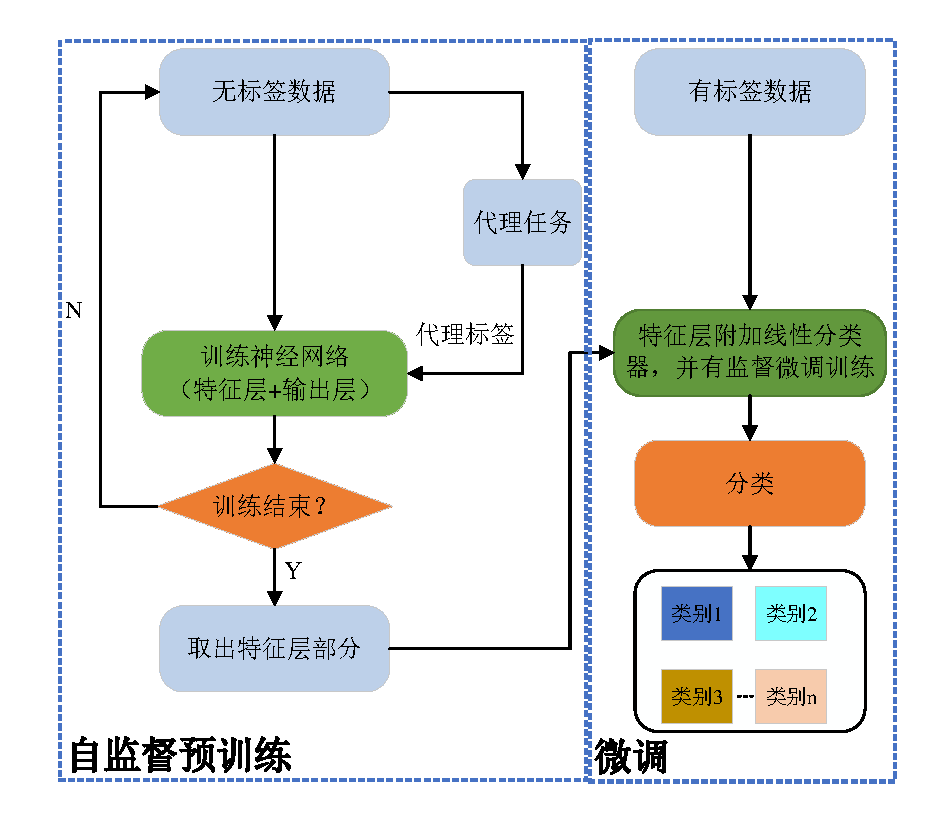
\includegraphics[width=10cm]{self_supervise_procedure.pdf}
    \caption{自监督训练范式流程}
    \label{self_supervise_procedure}
\end{figure}

(todo: 1.补充公式理论Rethinking the Value of Labels for Improving Class-Imbalanced Learning)
\section{孪生网络与对比学习相关理论}
对比学习是一种学习方法,侧重于通过对比正反两方面的实例来提取有意义的表征。它利用的假设是,在学习到的嵌入空间中,相似的实例应靠得更近,而不相似的实例应离得更远。通过将学习作为一项辨别任务,对比学习允许模型捕捉数据中的相关特征和相似性。对比学习主要分为监督对比学习和自监督对比学习两大类。

监督对比学习是对比学习的一个分支,它利用标记数据来明确训练模型以区分相似和不相似的实例。在监督对比学习中,模型在数据点对及其标签上进行训练,指示数据点是否相似或不相似。目标是学习一个表示空间,其中相似的实例聚集得更近,而不同的实例则被推开。一种流行的方法是信息噪声对比估计(InfoNCE)损失函数。 InfoNCE损失在学习的表示空间中最大化正样本之间的一致性并最小化负样本之间的一致性。通过优化此目标,模型学会区分相似和不相似的实例,从而提高下游任务的性能。

自监督对比学习采用不同的方法,从未标记的数据中学习表示,而不依赖于显式标签。 自监督对比学习利用借口任务的设计,从未标记的数据创建正负对。这些借口任务经过精心设计,旨在鼓励模型捕获数据中有意义的特征和相似性。自监督对比学习中常用的借口任务之一是生成增强视图。这涉及创建同一实例的多个增强版本并将它们视为正对,而来自不同样本的实例则被视为负对。通过训练模型来区分这些对,它可以学习捕获更高级别的语义信息并很好地推广到下游任务。
(todo:补充监督对比学习和自监督对比学习框图)
\section{相关数据集介绍}
\subsection{CWRU数据集介绍}
\begin{figure}
    \centering
    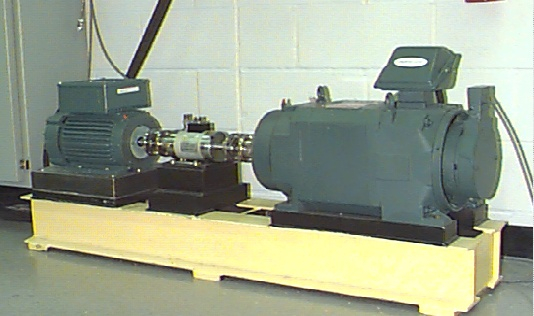
\includegraphics[width=6cm]{cwru_device.jpeg}
    \caption{CWRU轴承测试设备}
    \label{cwru_device}
\end{figure}
数据集由 CWRU(Case Western Reserve University)提供。图 \ref{cwru_device} 显示了测试设备,该设备包含一台 2 马力电机、一个扭矩编码器、一个测功机以及一些控制电路。测试使用的轴承为 6205-2RS JEM 深沟球轴承,分别安装在电机的驱动端和风扇端。  

轴承故障是通过单点电火花放电加工(Electro-discharge Machining)制造的。根据故障位置,故障类型可分为以下四种:  
1) 外圈故障(Outer Raceway Fault, OF);  
2) 内圈故障(Inner Raceway Fault, IF);  
3) 滚动体故障(Roller Faults, RFs);  
4) 正常状态(Normal Condition, NC)。  
轴承故障的严重程度可由故障直径(Fault Diameter)描述,故障直径指轴承或其他机械部件上出现的故障或损伤的直径尺寸。 故障直径通常用来描述故障的大小和程度,对于故障诊断和预测维护非常重要。

本研究采集了安装在驱动端的轴承数据,采样频率为 12 kHz,故障直径分别为 0.007 英寸,0.014英寸和0.021英寸的内圈故障、外圈故障、滚动体故障。不同故障类型的波形如图 \ref{cwru_samples} 所示。有关该数据集的更多详细信息,可访问 CWRU 轴承数据中心网站\citing{loparo2012case}。  

\begin{figure}
    \centering
    \subfloat[]{
        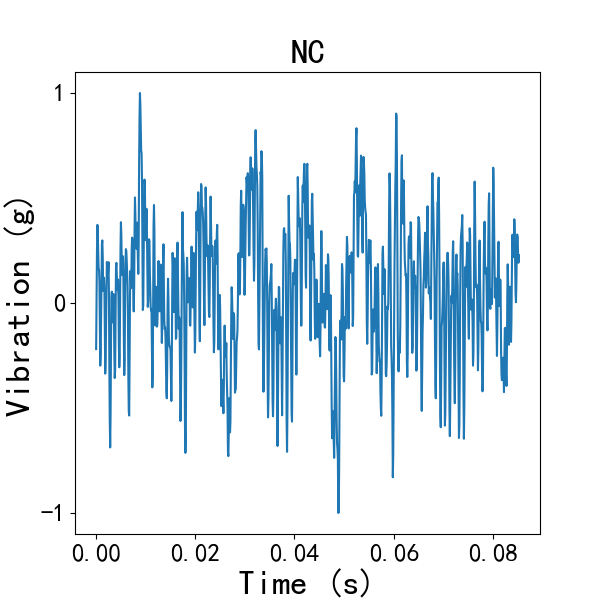
\includegraphics[width=0.28\linewidth]{class_0.png}
        \label{class_0}
    }
    \subfloat[]{
        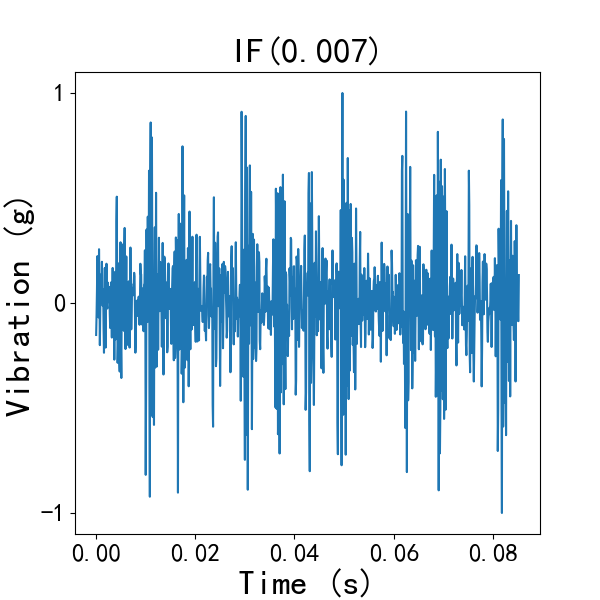
\includegraphics[width=0.28\linewidth]{class_1.png}
        \label{class_1}
    }
    \subfloat[]{
        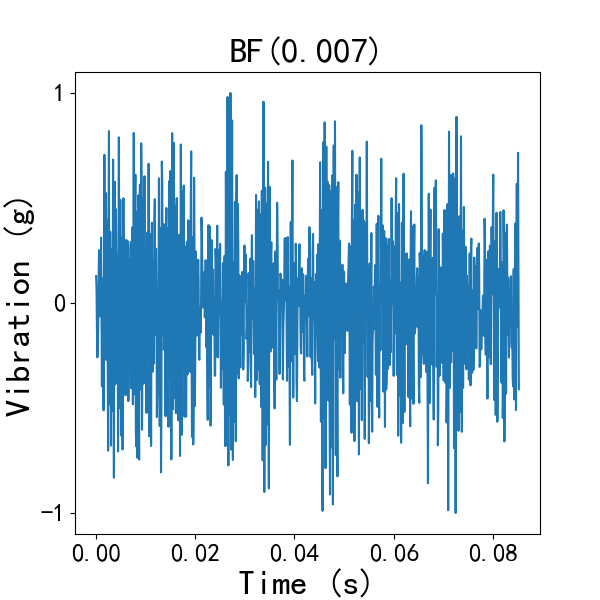
\includegraphics[width=0.28\linewidth]{class_2.png}
        \label{class_2}
    }
    \\ % 换行
    \subfloat[]{
        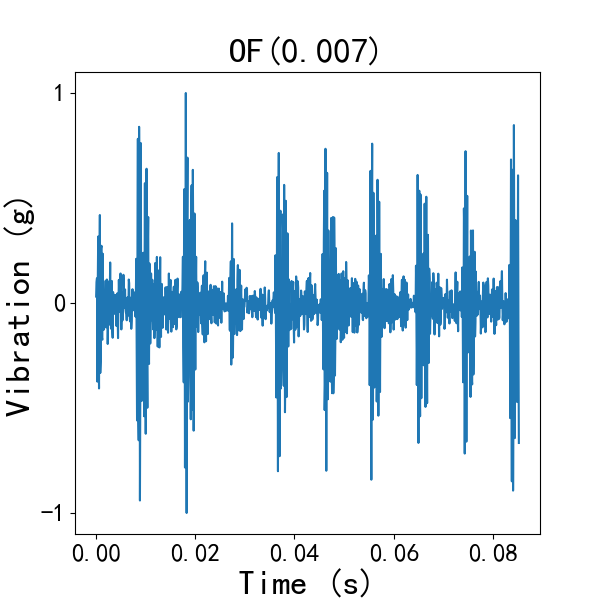
\includegraphics[width=0.28\linewidth]{class_3.png}
        \label{class_3}
    }
    \subfloat[]{
        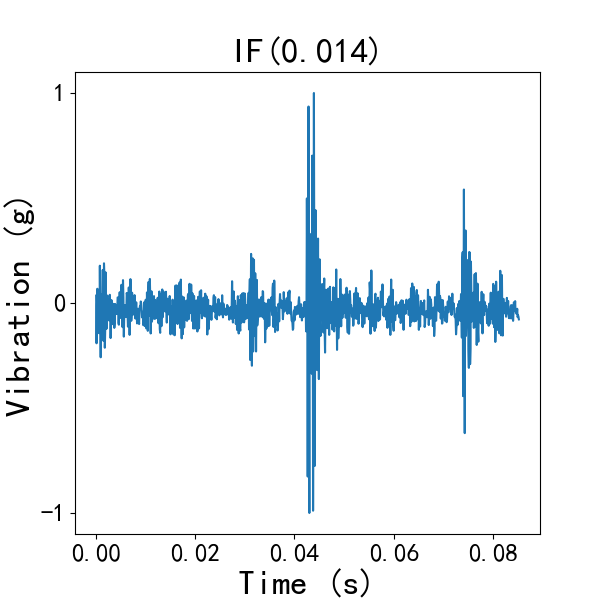
\includegraphics[width=0.28\linewidth]{class_4.png}
        \label{class_4}
    }
    \subfloat[]{
        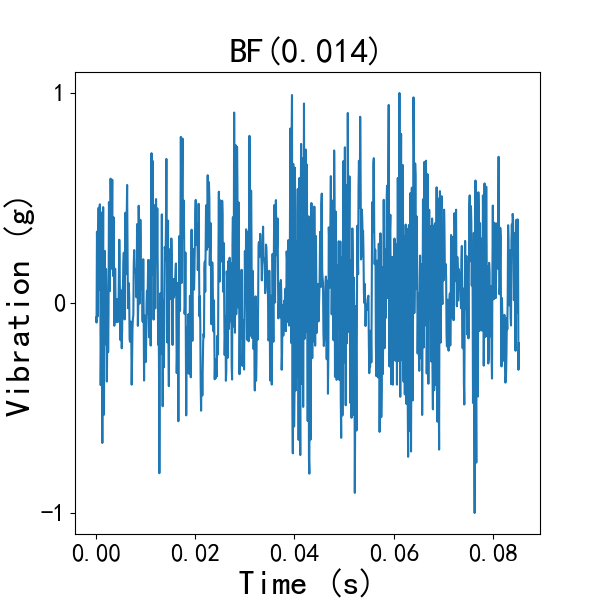
\includegraphics[width=0.28\linewidth]{class_5.png}
        \label{class_5}
    }
    \\ % 换行
    \subfloat[]{
        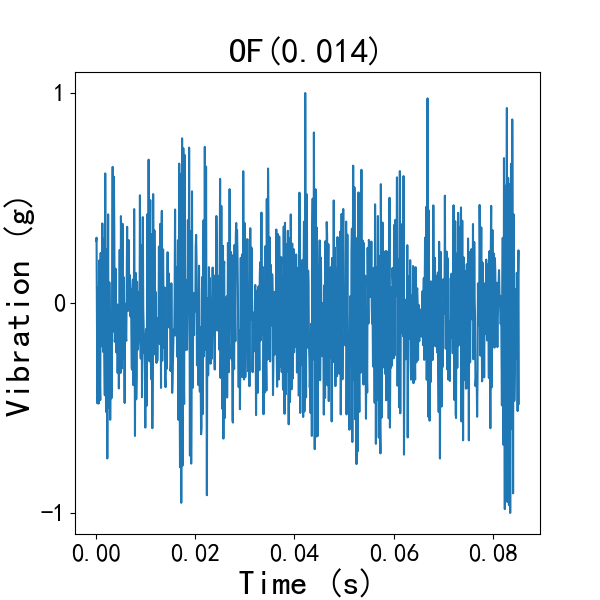
\includegraphics[width=0.28\linewidth]{class_6.png}
        \label{class_6}
    }
    \subfloat[]{
        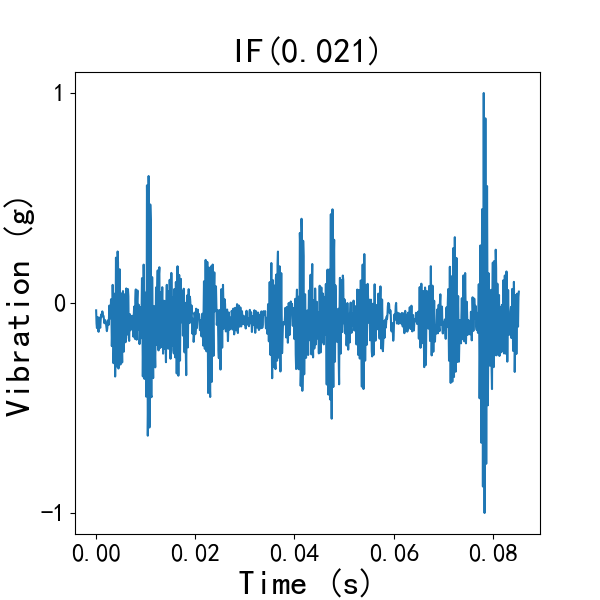
\includegraphics[width=0.28\linewidth]{class_7.png}
        \label{class_7}
    }
    \subfloat[]{
        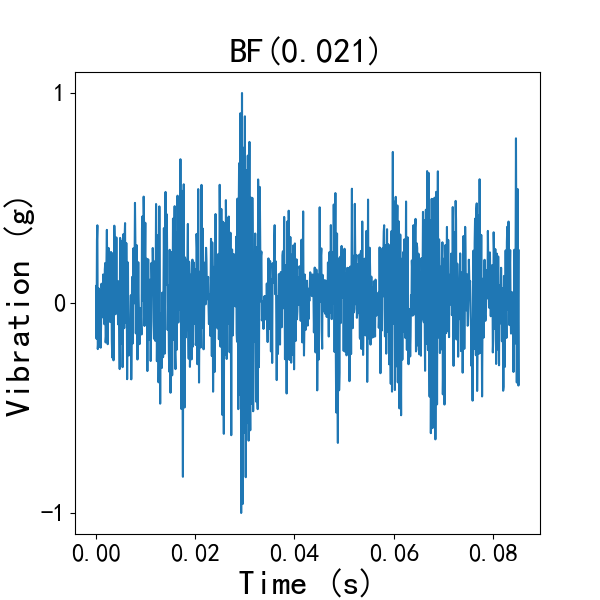
\includegraphics[width=0.28\linewidth]{class_8.png}
        \label{class_8}
    }
    \\ % 换行
    \subfloat[]{
        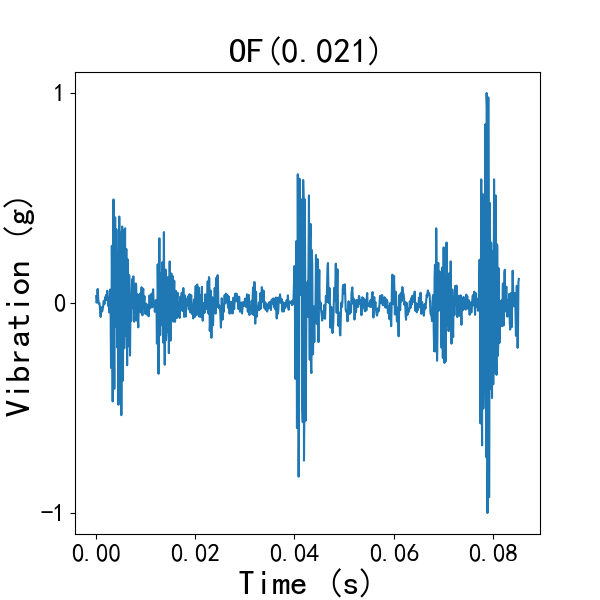
\includegraphics[width=0.28\linewidth]{class_9.png}
        \label{class_9}
    }

    \caption{每个类别的样本信号:\textbf{(a)} NC;\textbf{(b)} IF(0.007);\textbf{(c)} BF(0.007);\textbf{(d)} OF(0.007);\textbf{(e)} IF(0.014);\textbf{(f)} BF(0.014);\textbf{(g)} OF(0.014);\textbf{(h)} IF(0.021);\textbf{(i)} BF(0.021);\textbf{(j)} OF(0.021)。}
    \label{cwru_samples}
\end{figure}



\chapter{基于孪生网络对比学习的自监督预训练方法研究}
\section{模型整体架构及其模块设计}
\subsection{简单暹罗孪生网络}
\begin{figure}[h]
    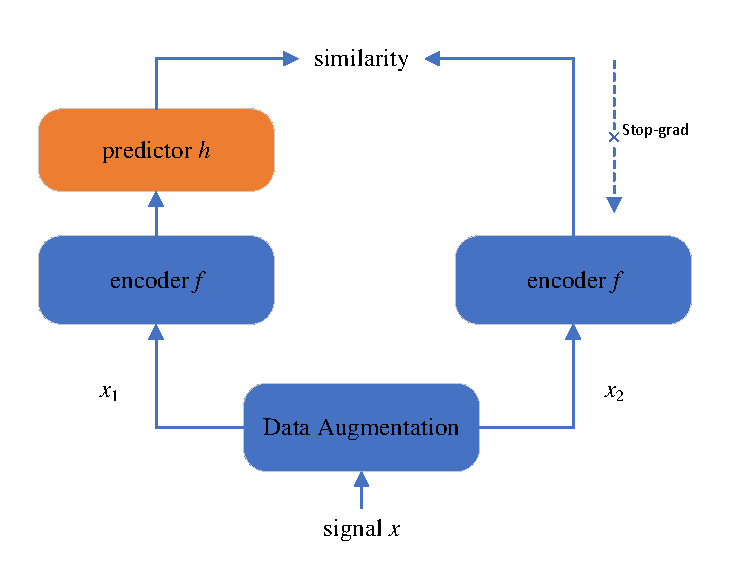
\includegraphics[width=12cm]{simsiam_arch.pdf}
    \caption{简单暹罗孪生网络}
    \label{simsiam_arch}
\end{figure}
简单暹罗孪生网络(SimSiam——Simple Siamese)\citing{chen2021exploring}架构(图\ref{simsiam_arch})将信号$x$中的两个随机增强视图$x_1$和$x_2$作为输入。这两个视图由编码器网络$f$处理,该网络由骨干网络(例如ResNet\citing{he2016deep})和投影MLP头部组成。编码器$f$在两个视图之间共享权重。预测MLP头部$h$转换一个视图的输出并将其与另一个视图进行匹配。将两个输出向量表示为$p_1 \triangleq h(f(x_1))$和$p_2 \triangleq f(x_2)$,我们最小化它们的负余弦相似度:
\begin{equation}
    \mathcal{D}(p_1, z_2) = -\frac{p_1}{\|p_1\|_2} \cdot \frac{z_2}{\|z_2\|_2}
    \label{eq:distance}
\end{equation}  
其中,$\|\cdot\|_2$ 是 $\ell_2$范数。定义对称损失函数
\begin{equation}
    \mathcal{L} = \frac{1}{2} \mathcal{D}(p_{1}, z_{2}) + \frac{1}{2} \mathcal{D}(p_{2}, z_{1})
\label{eq:cos_loss}
\end{equation}
该损失函数作用于单段信号,总损失值在计算所有信号的损失后取平均值。损失函数的最小值为-1。

方法中一个重要的组件是梯度停止(stop-grad)操作(图 1)。我们通过修改公式(\ref{eq:distance}) 来实现它:
\begin{equation}
    D(p_1, \text{stopgrad}(z_2))
\label{eq:stopgrad}
\end{equation}
这意味着在这一项中,\( z_2 \) 被视为常数。类似地,公式(\ref{eq:cos_loss}) 的实现形式为:
\begin{equation}
\mathcal{L} = \frac{1}{2} D(p_1, \text{stopgrad}(z_2)) + \frac{1}{2} D(p_2, \text{stopgrad}(z_1))
\label{eq:cos_loss_stopgrad}
\end{equation}
第一项中 \( x_2 \) 的编码器不会从 \( z_2 \) 接收梯度,但在第二项中会从 \( p_2 \) 接收梯度(反之亦然,对于 \( x_1 \) 也是如此)。即在这一项中,\( z_2 \) 被视为常数。

简单暹罗孪生网络的伪代码如表\ref{table:simsiam_code}所示。

\begin{table}
    \caption{简单暹罗孪生网络的伪代码,用Pytorch描述}
    \begin{tabular}{@{}l@{}} % 使用 @{} 去掉默认的左右边距,l 表示左对齐
    \toprule
    \multicolumn{1}{@{}l@{}}{\textbf{简单暹罗孪生网络Pytorch伪代码}} \\ % 左对齐文本
    \midrule
    \begin{lstlisting}[basicstyle=\ttfamily,frame=none]
#f: 骨干网络 + 投影 MLP
#h: 预测 MLP
for x in loader:  # 加载一个包含 n 个样本的小批量数据 x
    x1, x2 = aug(x), aug(x)  # 随机数据增强
    z1, z2 = f(x1), f(x2)  # 投影,形状为 n-by-d
    p1, p2 = h(z1), h(z2)  # 预测,形状为 n-by-d
    L = D(p1, z2)/2 + D(p2, z1)/2  # 损失函数

    L.backward()  # 反向传播
    update(f, h)  # SGD 更新

def D(p, z):  # 负余弦相似度
    z = z.detach()  # 停止梯度
    p = normalize(p, dim=1)  # 对 p 进行 L2 归一化
    z = normalize(z, dim=1)  # 对 z 进行 L2 归一化
    return -(p * z).sum(dim=1).mean()  # 计算负余弦相似度
    \end{lstlisting} \\
    \bottomrule
    \end{tabular}
    \label{table:simsiam_code}
\end{table}
\subsection{简单暹罗孪生故障诊断网络}
\begin{figure}[h]
    \centering
    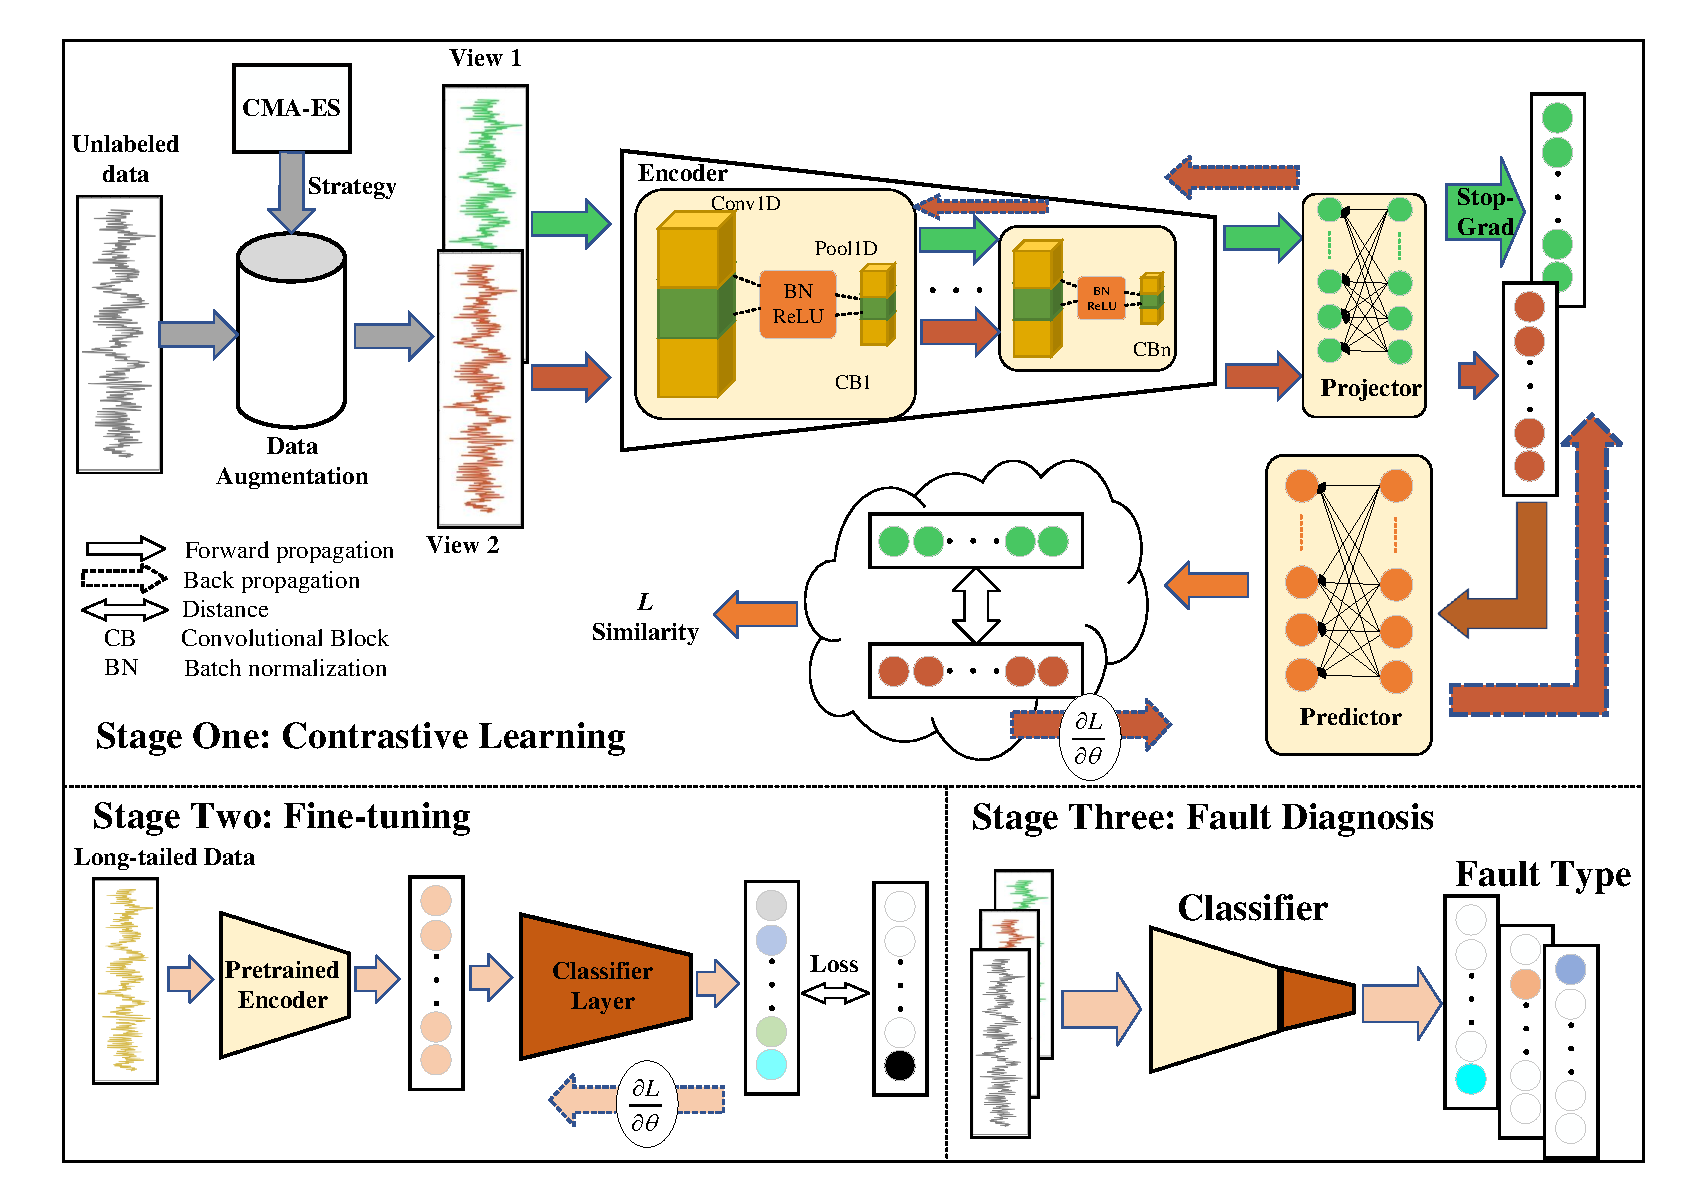
\includegraphics[width=16cm]{simsiam_net.pdf}
    \caption{简单暹罗孪生故障诊断网络}
    \label{simsiam_net}
\end{figure}
提出的用于故障诊断的简单暹罗孪生网络如图\ref{simsiam_net}所示,以下是架构的介绍。

1)\textbf{数据增强(Data Augmentations)}:
在对比表示学习算法中,数据增强(DA)起着至关重要的作用。成功地从振动信号中提取可区分的故障特征,依赖于为同一样本生成不同视图的质量。我们知道,面向图像的最新(SOTA)对比表示学习算法广泛使用多种数据增强方法,而针对序列数据的增强方法则相对较少。
此外,用于对比学习生成正样本对的增强方法必须满足一个条件,即加入样本的噪声不能改变其语义含义。因此,我们选择了以下九种数据增强方法:

\begin{itemize}
    \item \textbf{掩码(Random Masked)}:用于遮盖输入数据的一部分,即随机挑选信号的某些部分用 0 替代,通常是在序列数据或图像数据中随机选择部分区域进行掩码处理。这有助于模型在训练时学会忽略一些无关信息,从而提高其鲁棒性。

    \item \textbf{添加高斯噪声(Adding Gaussian Noise)}:将高斯噪声添加到数据中的方法,常用于增强模型的鲁棒性。通过这种方式,模型在训练过程中能够适应噪声,并提升其在实际应用中的性能,尤其是在存在噪声的环境中。

    \item \textbf{相位扰动(Phase Perturbation)}:修改信号的频率域中的相位信息,而保持幅度不变来生成新的数据样本。这种方法保留了信号的整体结构,但引入了细微的扰动,用于提高模型的泛化能力。

    \item \textbf{块打乱(RandomChunkShuffle)}:将时间序列数据分割成多个块,然后随机打乱这些块的顺序。这样可以创建不同的序列变体,增加模型对数据变异的适应能力,同时保持整体的语义不变。

    \item \textbf{随机缩放(Random Scaled)}:对数据进行随机幅度缩放来增强数据的方法。通过改变数据的尺度,模型能够学习到不同幅度下的数据模式,从而提升其泛化能力。

    \item \textbf{随机绝对值(Random Abs)}:对数据应用绝对值操作,将负值转换为正值或去掉负号。这个方法帮助模型处理包含负值的情形,增强其鲁棒性。

    \item \textbf{竖直翻转(Random Vertical Flip)}:随机地将数据进行竖直翻转来创建新的样本。这对于一些对竖直方向变化不敏感的任务非常有效。

    \item \textbf{水平翻转(Random Horizontal Flip)}:随机将图像或数据进行水平翻转,生成新的样本。这种方法对于对称性较强的数据非常有效,能增强模型的鲁棒性。

    \item \textbf{时移(Time Shift)}:将数据在时间轴上平移一定的时间步长来生成新的样本。这种方法可以帮助模型学会适应时间序列数据中事件的变化位置,提升其对时间依赖的理解能力。
\end{itemize}

同一输入信号分别经过上述数据增强方法后的视图如图\ref{data_augmentation}所示。
\begin{figure}[h]
    \centering
    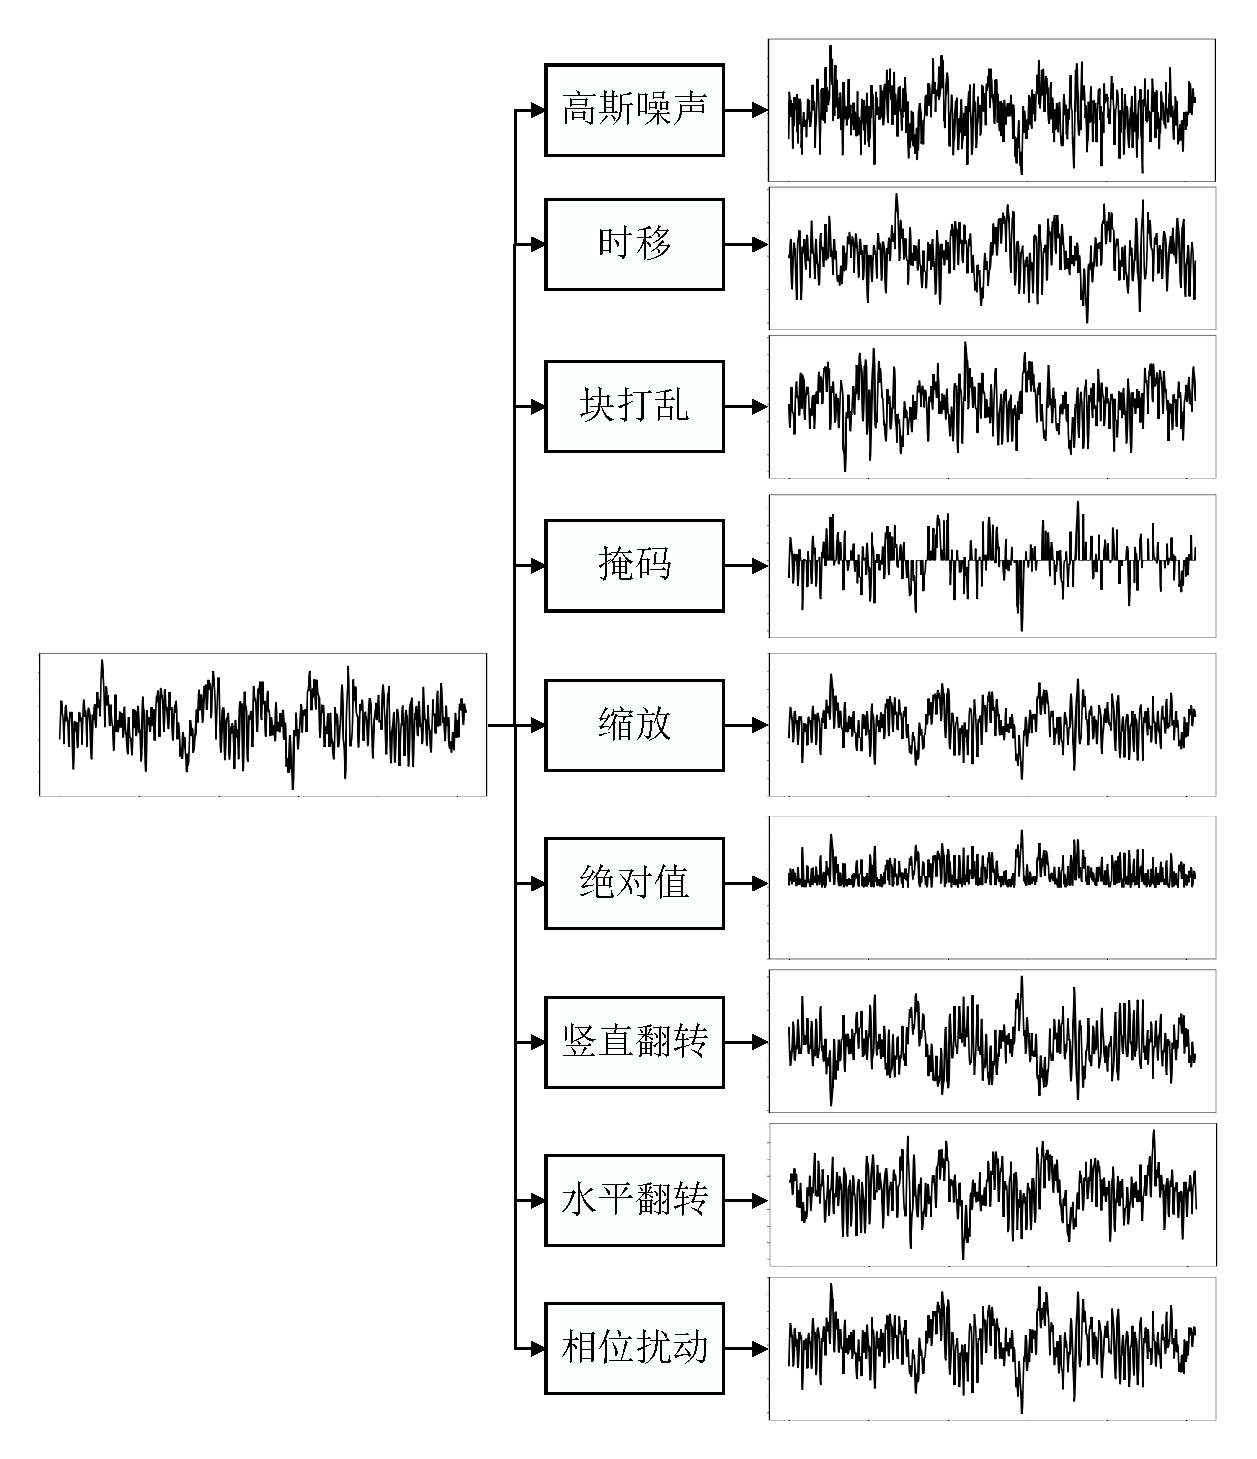
\includegraphics[width=10cm]{data_augmentation.pdf}
    \caption{数据增强示意图}
    \label{data_augmentation}
\end{figure}

2)\textbf{编码器(Encoder),预测器(Predictor)和分类器(Classifier)}:编码器是该算法中故障诊断的关键部分。我们主要使用其潜在编码来完成分类任务。由于简单暹罗网络是一个框架,我们可以根据需要构建编码器模型和预测器,其中预测器是一个相对简单的非线性函数。在第二阶段,需要在预训练的编码器后添加一个分类器层用于故障诊断,如图\ref{simsiam_net}所示。为了方便起见,我们使用多个常规的卷积神经网络(CNN)块来构建编码器,并使用全连接层来构建预测器和分类器。每个卷积块(CB)包括四个层:一个 1-D 卷积层\( f_{\text{BN}} \)、一个激活函数层 \( f_{\text{ReLU}} \),以及一个池化层 \( f_{\text{Pool}} \)。 方程(\ref{eq:CNN})展示了 1-D 卷积层的操作,其中输入的形状为 \( (N, C_{\text{in}}, L) \),输出的形状为 \( (N, C_{\text{out}}, L_{\text{out}}) \),其中 \( N \) 是样本的数量,\( C \) 表示通道数,\( L \) 表示数据的长度。
\begin{equation}
    \begin{aligned}
    \operatorname{out}(N_i, C_{\mathrm{out}_j}) &= \operatorname{bias}(C_{\mathrm{out}_j}) + \sum_{k=0}^{C_{\mathrm{in}}-1} \operatorname{weight}(C_{\mathrm{out}_j}, k) \otimes \operatorname{input}(N_i, k).
    \end{aligned}
    \label{eq:CNN}
    \end{equation}
BN 层 \( f_{\text{BN}} \) 用于加速训练过程并减少由于层输入分布不同而导致的内部协变量偏移(ICS)的影响 \citing{ioffe2015batch},当模型较深时,这种影响尤为严重。公式(\ref{eq:BN})展示了批归一化的过程。
\begin{equation}
    f_{\text{BN}}(x_i, \mathbf{x}) = \gamma \frac{x_i - \mathbb{E}(\mathbf{x})}{\sqrt{\sigma(\mathbf{x})^2 + \epsilon}} + \beta
\label{eq:BN}
\end{equation}    
\begin{equation}
\mathbb{E}(\mathbf{x}) = \frac{1}{N}\sum_{i=1}^N x_i
\label{eq:exp_BN}
\end{equation}
\begin{equation}
\sigma(\mathbf{x}) = \sqrt{\frac{1}{N}\sum_{i=1}^N (x_i - \mathbb{E}(\mathbf{x}))^2}
\label{eq:sigma_BN}
\end{equation}
其中 \( x \) 是整个小批量(mini batch)的向量,批量大小为 \( N \),\( x_i \) 表示小批量中的第 \( i \) 个样本。  
\( \mathbb{E}(x) \) 和 \( \sigma(x) \) 分别表示向量批量的均值和方差,如公式 (\ref{eq:exp_BN}) 和 (\ref{eq:sigma_BN}) 所示。\( \epsilon \) 是一个超参数,通常设置为 \( 10^{-5} \),而 \( \gamma \) 和 \( \beta \) 分别是缩放因子和偏移因子,它们是可学习的参数,初始值分别设置为 1 和 0。

激活层 \( f_{\text{ReLU}} \) 可以表示为公式 (\ref{eq:relu}):
\begin{equation}
    f_{\text{ReLU}} = \max(0, x)
    \label{eq:relu}
\end{equation}

\( x_i^{(n)} \) 表示通过第 \( n \) 个卷积块(CB)的第 \( i \) 个输出向量,可以用公式 (\ref{eq:output_of_encoder}) 表示:
\begin{equation}
    \begin{aligned}
    x_i^{(n)} = f_{\text{Pool}}\bigl\{f_{\text{ReLU}}\bigl[f_{BN}\Bigl(f_{\text{conv}}\bigl(\mathbf{x}^{(n-1)}\bigr), f_{\text{conv}}\Bigl(x_i^{(n-1)}\Bigr)\Bigr)\bigr]\bigr\}
    \end{aligned}
    \label{eq:output_of_encoder}
\end{equation}

3)\textbf{优化器(Optimizer)}:模型的训练不需要使用大批量优化器,例如分层自适应速率缩放(LARS)\citing{you2017large},因为所提出的方法可以在典型批量大小下工作,而不依赖于大批量训练。我们使用 SGD 优化器训练模型。网络参数通过公式 (\ref{eq:SGD}) 更新。
\begin{equation}
    \theta_{l+1} = \theta_l - \eta_l \cdot \nabla_{\theta} \mathcal{L}(\mathbf{x}; \theta_l)
\label{eq:SGD}
\end{equation}
其中 \( \theta_t \) 表示时间 \( t \) 时的可学习参数,\( \eta_t \) 表示时间 \( t \) 时的学习率,\( L(\cdot) \) 表示损失函数。

4)\textbf{微调(Fine-tuning)}:在对比学习阶段完成后,我们从模型中取出训练好的编码器 \( f \),并将其与一个多层感知器(MLP)模块连接,我们用带标签的数据微调构建一个完整的分类器用于故障诊断任务,从而使模型获得分类能力。以准确率为性能指标,如公式 (\ref{eq:acc}):
\begin{equation}
    \text{Accuracy} = \frac{TN + TP}{TN + TP + FP + FN}
    \label{eq:acc}
\end{equation}
其中,\( TN \) 表示真阴性,即被正确预测为阴性的阴性样本数量。真阳性(\( TP \))表示被模型正确判断为阳性的阳性样本数量。假阳性(\( FP \))表示被错误分类为阳性的阴性样本数量。假阴性(\( FN \))表示被错误分类为阴性的阳性样本数量。  

当验证集的样本均匀采样后(本研究采用此方法),准确率等于宏平均召回率(Macro-Averaged Recall)。宏平均召回率是对每个类别单独计算召回率,然后取平均值:
\begin{equation}
    \text{Macro-Recall} = \frac{1}{C} \sum_{i=1}^{C} \frac{TP_i}{TP_i + FN_i}
    \label{eq:macro_recall}
\end{equation}
其中,\( C \) 是类别的总数,\( TP_i \) 和 \( FN_i \) 分别是第 \( i \) 类的真正例和假负例。




5)\textbf{故障诊断(Fault Diagnosis)}:在完成微调后,即可将模型应用于真实输入信号的故障诊断,以预测故障类别。
\begin{figure}[h]
    \centering
    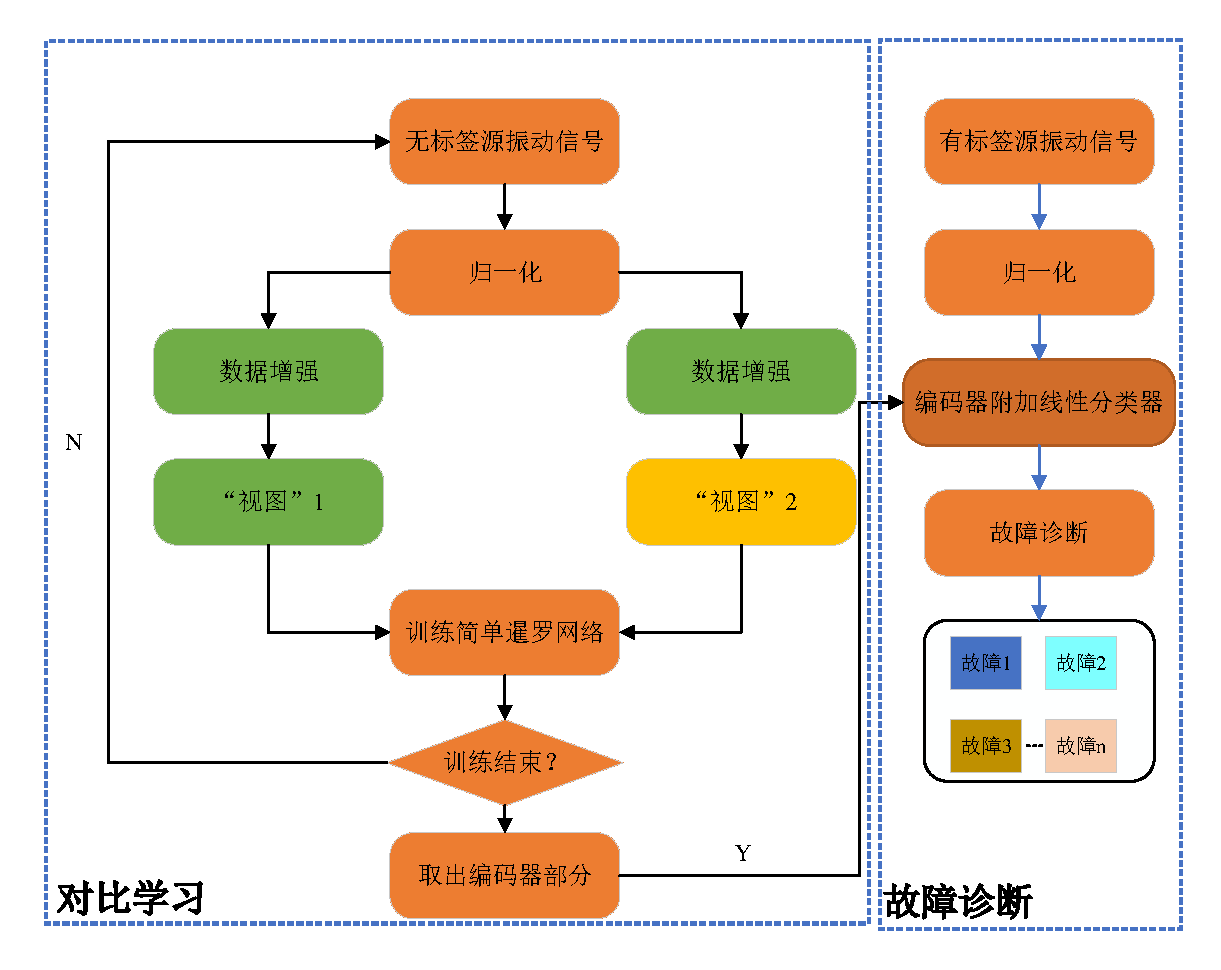
\includegraphics[width=14cm]{simsiam_fault_diag_procedure.pdf}
    \caption{简单暹罗孪生故障诊断网络的训练流程图}
    \label{simsiam_fault_diag_procedure}
\end{figure}
简单暹罗孪生故障诊断网络的训练过程如图\ref{simsiam_fault_diag_procedure}所示。首先,我们需要对所有未标记的振动样本进行归一化预处理,并使用数据增强方法生成输入样本的两个不同视图作为正样本对。我们将正样本对输入模型,然后按照算法表\ref{table:simsiam_code}所示的流程训练模型。训练过程完成后,我们取出编码器,在其最后一层后附加一个线性分类层,并使用标记样本对模型进行微调。线性分类层也可以用其他分类器(如 K 近邻(KNN)和支持向量机(SVM))替换。

\subsection{基于CMA-ES优化器的最优数据增强策略搜索算法}
简单暹罗孪生网络的一个难以接受的平凡解是所有输出都“坍塌”为一个常数。简单暹罗孪生网络利用数据增强生成两个视图,并直接最大化同一输入的两个视图的相似性,即不使用负样本对。因此简单暹罗孪生网络极大程度上依赖于数据增强的效果,而人工筛选数据增强十分耗时耗力且难以获得最优解。该节提出了基于CMA-ES优化器的最优数据增强策略搜索算法,CMA-ES(Covariance Matrix Adaptation Evolution Strategy,协方差矩阵自适应进化策略)是一种用于连续优化问题的进化算法。它是一种基于种群的优化方法,通过自适应调整协方差矩阵来指导搜索方向,从而在高维空间中高效地找到全局最优解。CMA-ES 在解决非线性、非凸、高维优化问题时表现出色,广泛应用于机器学习、工程优化和科学研究中。CMA-ES 的更新规则如下:

1. 采样新解:
\begin{equation}
\mathbf{x}_k^{(g+1)} = \mathbf{m}^{(g)} + \sigma^{(g)} \cdot \mathcal{N}(0, \mathbf{C}^{(g)})
\label{eq:sample}
\end{equation}
其中:
\begin{itemize}
    \item \(\mathbf{x}_k^{(g+1)}\) 是第 \(g+1\) 代中的第 \(k\) 个候选解,
    \item \(\mathbf{m}^{(g)}\) 是第 \(g\) 代的均值向量,
    \item \(\sigma^{(g)}\) 是第 \(g\) 代的步长,
    \item \(\mathbf{C}^{(g)}\) 是第 \(g\) 代的协方差矩阵,
    \item \(\mathcal{N}(0, \mathbf{C}^{(g)})\) 是从多元正态分布中采样的随机向量。
\end{itemize}

2. 更新均值:
\begin{equation}
\mathbf{m}^{(g+1)} = \sum_{i=1}^{\mu} w_i \mathbf{x}_{i:\lambda}^{(g+1)}
\label{eq:mean_update}
\end{equation}
其中:
\begin{itemize}
    \item \(\mu\) 是选择的父代数量,
    \item \(w_i\) 是权重系数,
    \item \(\mathbf{x}_{i:\lambda}^{(g+1)}\) 是第 \(g+1\) 代中适应度排名前 \(\mu\) 的候选解。
\end{itemize}

3. 更新协方差矩阵:
\begin{equation}
\mathbf{C}^{(g+1)} = (1 - c_1 - c_\mu) \mathbf{C}^{(g)} + c_1 \mathbf{p}_c^{(g+1)} (\mathbf{p}_c^{(g+1)})^\top + c_\mu \sum_{i=1}^{\mu} w_i \mathbf{y}_{i:\lambda}^{(g+1)} (\mathbf{y}_{i:\lambda}^{(g+1)})^\top
\label{eq:covariance_update}
\end{equation}
其中:
\begin{itemize}
    \item \(c_1\) 和 \(c_\mu\) 是学习率,
    \item \(\mathbf{p}_c^{(g+1)}\) 是进化路径,
    \item \(\mathbf{y}_{i:\lambda}^{(g+1)} = (\mathbf{x}_{i:\lambda}^{(g+1)} - \mathbf{m}^{(g)}) / \sigma^{(g)}\)。
\end{itemize}

4. 更新步长:
\begin{equation}
\sigma^{(g+1)} = \sigma^{(g)} \exp\left(\frac{c_\sigma}{d_\sigma} \left(\frac{\|\mathbf{p}_\sigma^{(g+1)}\|}{\mathbb{E}[\|\mathcal{N}(0, \mathbf{I})\|]} - 1\right)\right)
\label{eq:stepsize_update}
\end{equation}
其中:
\begin{itemize}
    \item \(c_\sigma\) 是步长学习率,
    \item \(d_\sigma\) 是阻尼系数,
    \item \(\mathbf{p}_\sigma^{(g+1)}\) 是步长进化路径,
    \item \(\mathbb{E}[\|\mathcal{N}(0, \mathbf{I})\|]\) 是标准正态分布向量的期望范数。
\end{itemize}

我们将寻找最佳数据增强策略的问题形式化为一个搜索问题(见图 \ref{CMA-ES})。我们的方法由两个组件组成:搜索算法和搜索空间。在高层次上,搜索算法(实现为CMA-ES)采样一个数据增强策略 \( S \),该策略包含有关使用哪种图像处理操作、每批次中使用该操作的概率以及操作幅度的信息。我们方法的关键在于,策略 \( S \) 将用于训练具有固定架构的神经网络,其验证准确率 \( R \) 将返回以评估适应度。
\begin{figure}[h]
    \centering
    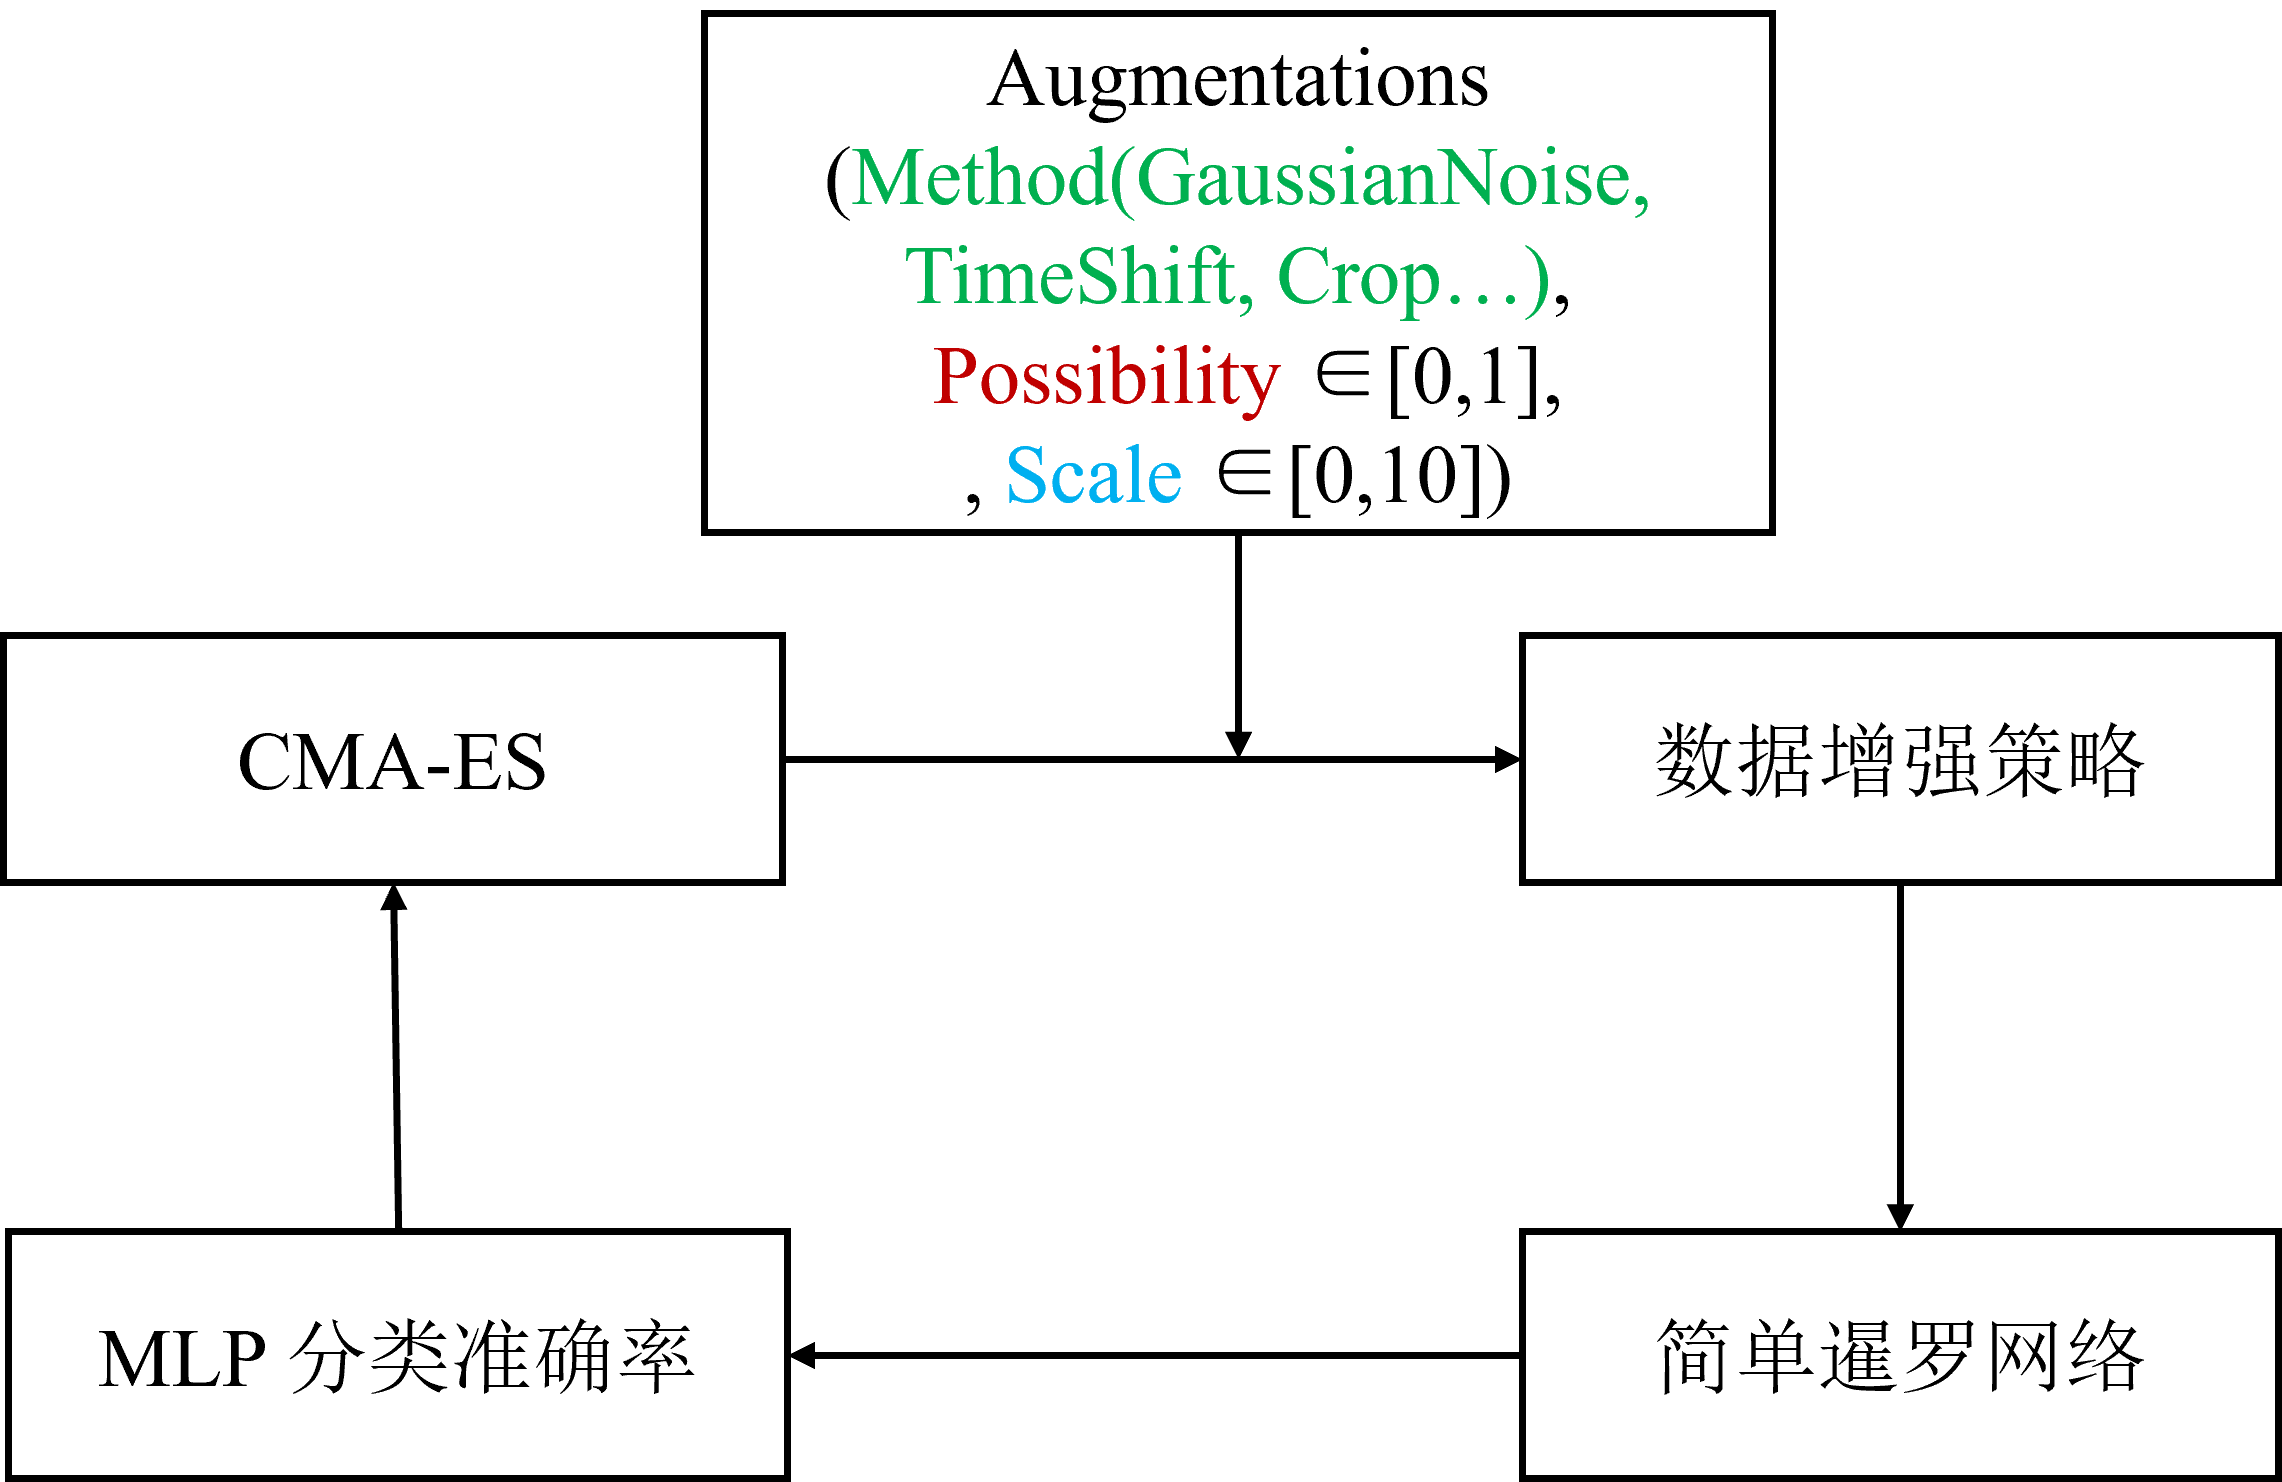
\includegraphics[width=8cm]{CMA-ES.png}
    \caption{使用CMA-ES搜索最优的数据增强策略框架概览}
    \label{CMA-ES}
\end{figure}
搜索空间细节:在我们的搜索空间中,一个策略由 8 个信号数据增强子策略组成,如图\ref{data_augmentation}所示。此外,每个操作还关联两个超参数:
\begin{itemize}
    \item 1) 应用操作的概率\(\in [0,1]\),
    \item 2) 操作的幅度映射后\(\in [0,10]\)。
\end{itemize}
映射为线性变换,如变量\(x \in [a,b]\)到\(y \in [0,10]\)的变换为
\begin{equation}
    y = \frac{10(x - a)}{b - a}
    \end{equation}
以下介绍各个数据增强子策略幅度的表示:
\begin{itemize}
    \item \textbf{掩码(Random Masked)}:随机选取100个不重叠的大小为$s$的子区间,将其置0。$s$作为增强幅度由\([1,5]\)映射为\([0,10]\)。

    \item \textbf{添加高斯噪声(Adding Gaussian Noise)}:将高斯噪声的信噪比SNR作为增强幅度,由\([2,6]\)映射为\([0,10]\)。

    \item \textbf{相位扰动(Phase Perturbation)}:相位扰动服从均匀分布$\text{U}(-perturb_{\text{max}}, perturb_{\text{max}})$,$perturb_{\text{max}}$作为增强幅度由\([0.1,0.5]\)映射为\([0,10]\)。

    \item \textbf{块打乱(RandomChunkShuffle)}:将时间序列数据分割成大小均匀的$s$个块,然后随机打乱这些块的顺序。$s$作为增强幅度由\([10,100]\)映射为\([0,10]\)。

    \item \textbf{随机缩放(Random Scaled)}:缩放的幅度服从均匀分布$\text{U}(1.0-scale, 1.0+scale)$。$scale$作为增强幅度由\([0.05,0.6]\)映射为\([0,10]\)。

    \item \textbf{随机绝对值(Random Abs)}:无幅度值。

    \item \textbf{竖直翻转(Random Vertical Flip)}:无幅度值。

    \item \textbf{水平翻转(Random Horizontal Flip)}:无幅度值。
    
\end{itemize}
则CMA-ES优化器求解的问题可以描述为 
\begin{equation}
    \arg\max_{\mathbf{p}, \mathbf{s}} \text{Accuracy}(\mathbf{p}, \mathbf{s}, \text{SimSiam-Net})
\end{equation}
其中,\(\mathbf{p}\) 和 \(\mathbf{s}\) 为求解的参数,分别满足 \(p_i \in [0, 1]\) 和 \(s_i \in [0, 10]\),Accuracy为简单暹罗网络验证的准确率。

\section{实验与分析}
为了验证所提出方法的有效性,我们选择了三种不同的轴承故障数据进行实验。它们分别是 CWRU 数据集、SQ 数据集和 PB 数据集。此外,为了证明所提出方法的优越性,我们选择了几种流行的方法作为对比方法,这些方法可以分为两类。一类是传统的机器学习算法,另一类是当前基于深度学习的智能方法。对比方法如下所示。
\begin{enumerate}
    \item \textbf{SVM [31]}:多类 SVM 是一种强大且多功能的机器学习模型,能够执行线性或非线性分类任务。首先,我们将计算原始数据的 16 个时域指标(均值、平方根、偏度等),并将它们作为 SVM 分类器的输入。

    \item \textbf{CNN [32]}:CNN 是一种监督学习方法。在这里,CNN 的网络架构与所提出方法的编码器 \(f\) 相同。

    \item \textbf{LiftingNet [33]}:一种监督学习方法,其中应用了分层特征学习,网络架构与原始文章保持一致。

    \item \textbf{Multiscale [34]}:一种监督学习方法,其中模型采用了多尺度特征提取单元。网络架构与原始文章保持一致。

    \item \textbf{多感受野图卷积网络 (MRF-GCN) [35]}:一种使用多感受野图卷积网络 (GCN) 的监督学习轴承故障诊断方法,采用两阶段训练策略。

    \item \textbf{快速自注意力卷积生成对抗网络 (QSCGAN) [36]}:QSCGAN 是一种新颖的半监督生成对抗网络,用于故障诊断,采用两阶段训练策略。模型与原始文章保持一致。

    \item \textbf{BYOL [27]}:BYOL 也是一种自监督表示学习方法,它依赖于两个相互交互和学习的神经网络块。编码器 \(f\) 和数据增强方法与所提出方法相同。
\end{enumerate}
\subsection{简单暹罗孪生网络实现细节}
由于简单暹罗网络是一个框架,我们可以根据需要构建编码器模型和预测器,以下介绍本文构建的简单暹罗网络框架的细节。
\begin{itemize}
    \item \textbf{Encoder}:堆叠了十个 CNN 块作为编码器,其中卷积层的核大小设置为 3,填充设置为 1,步幅设置为 1,隐藏层采用 256 个核。
    
    \item \textbf{Predictor}:我们使用两个线性全连接层构建预测器,分别具有 \( 256 \times 512 \) 和 \( 512 \times 256 \) 个神经元。我们在它们之间放置了一个批归一化层和一个修正线性单元(ReLU)层。

    \item \textbf{Classifier}:至于分类器层,我们也部署了两个线性全连接层,分别具有 \( 256 \times 256 \) 和 \( 256 \times \text{num\_class} \) 个神经元,其中 \(\text{num\_class}\) 表示故障类别的数量。在两个线性层之间也放置了一个批归一化层和一个 ReLU 层。

    \item \textbf{Optimizer}:
        优化器为 SGD 优化器,其学习率初始设置为 \( 0.05 \times \frac{\text{BatchSize}}{256} \),学习率采用余弦衰减调度。余弦衰减调度的公式为:
        \[
        \eta_t = \eta_{\text{min}} + \frac{1}{2} (\eta_{\text{max}} - \eta_{\text{min}}) \left(1 + \cos\left(\frac{t \pi}{T}\right)\right)
        \]
        其中:
        \begin{itemize}
            \item \(\eta_t\) 是第 \(t\) 步的学习率,
            \item \(\eta_{\text{max}}\) 是初始学习率(最大学习率),
            \item \(\eta_{\text{min}}\) 是最小学习率,
            \item \(t\) 是当前训练步数,
            \item \(T\) 是总训练步数(衰减周期),
            \item \(\cos\) 是余弦函数。
        \end{itemize}
        权重衰减为 0.0001,SGD 动量为 0.9。

    \item \textbf{损失函数}:对比学习预训练阶段的损失函数为余弦相似度见\ref{eq:distance},微调阶段的损失函数为交叉熵损失函数(Cross-Entropy Loss Function)。对于多分类问题,交叉熵损失函数表示为
    \begin{equation}
        \mathcal{L}_{\text{CE}} = -\sum_{i=1}^{C} y_i \log(\hat{y}_i)
        \end{equation}        
        其中:
        \begin{itemize}
            \item \( C \) 是类别数量,
            \item \( y_i \) 是真实标签的 one-hot 编码(第 \( i \) 类的真实概率),
            \item \( \hat{y}_i \) 是模型预测的第 \( i \) 类的概率。
        \end{itemize}

    \item \textbf{长尾分布数据集模拟构造}:模拟构建长尾分布数据集流程如图\ref{pareto}所示。设定不平衡因子 \(\beta = x_{\text{max}} / x_{\text{min}}\) 为数据集中样本数量最多的类与样本数量最少的类的数量之比。帕累托分布的概率密度函数为 \(p(x) = \frac{\alpha x_{\text{min}}^{\alpha}}{x^{\alpha+1}}\),令$x_{\text{min}} = 1$,则\(p(x) = \frac{\alpha}{x^{\alpha+1}}\)。以不平衡因子构建服从帕累托分布的长尾分布数据集,不同不平衡因子的帕累托分布概率密度函数如图\ref{paerto_fig_beta}所示,可以看到当最大类与最小类样本数的比值 \(\beta\) 增大时,帕累托分布的形状参数 \(\alpha\) 也随之增大。这表明分布的头部类别占比提高,而尾部类别占比显著降低,长尾效应越发显著。下面将介绍形状参数 \(\alpha\) 的求解方法,以及各类别样本占比的计算步骤。

    \begin{figure}[h]
        \centering
        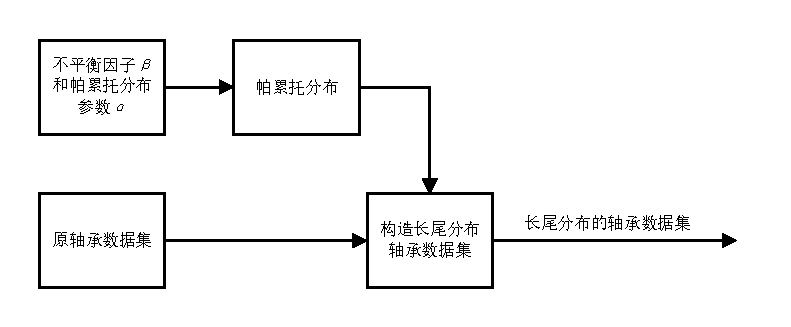
\includegraphics[width=12cm]{pareto.pdf}
        \caption{基于帕累托分布构造长尾分布的轴承数据集流程图}
        \label{pareto}
    \end{figure}

    \begin{figure}[h]
        \centering
        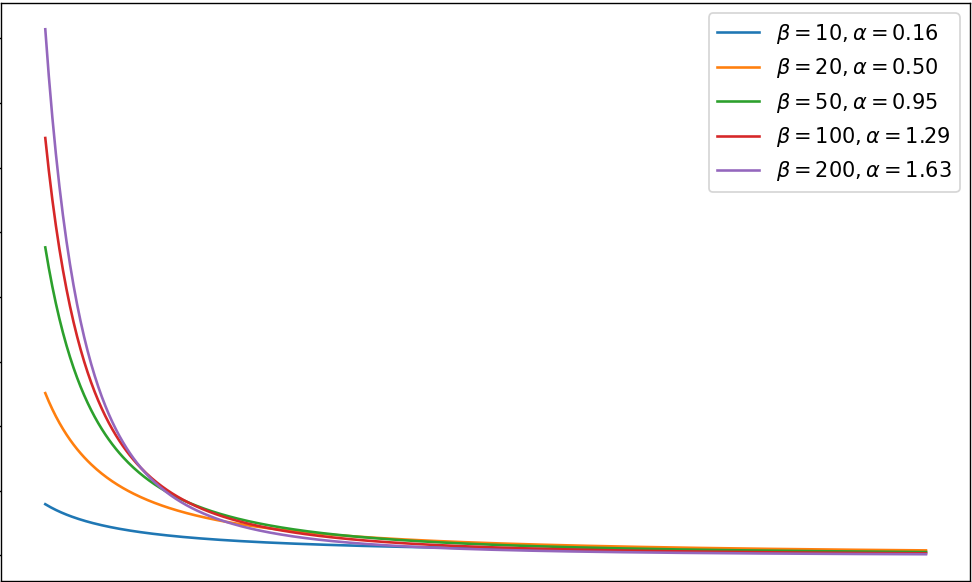
\includegraphics[width=12cm]{paerto_fig_beta.png}
        \caption{不同$\beta$的帕累托分布概率密度图}
        \label{paerto_fig_beta}
    \end{figure}

    已知帕累托分布的累积分布函数为:
    \begin{equation}
    F(x) = 1 - x^{-\alpha}, \quad x > 1
    \end{equation}

    每类的概率定义为:
    \begin{equation}
    P(n \leq x < n+1) = F(n+1) - F(n) = n^{-\alpha} - (n+1)^{-\alpha}
    \end{equation}

    设最大类与最小类的样本数比值为 $\beta$,则有以下关系式:
    \begin{equation}
    \beta = \frac{P(1 \leq x < 2)}{P(n \leq x < n+1)} = \frac{1 - 2^{-\alpha}}{n^{-\alpha} - (n+1)^{-\alpha}}
    \end{equation}

    目标是:
    \begin{enumerate}
        \item 根据给定的 $\beta$ 和类别总数 $n$,求解形状参数 $\alpha$。
        \item 计算每类的样本占比 $P(n \leq x < n+1)$。
        \item 将所有类别的概率归一化,使其和为 1。
    \end{enumerate}

    具体步骤:

    \begin{enumerate}
        \item \textbf{求解 $\alpha$} \\
        根据 $\beta$ 的定义,解以下非线性方程以确定 $\alpha$:
        \begin{equation}
        \beta = \frac{1 - 2^{-\alpha}}{n^{-\alpha} - (n+1)^{-\alpha}}
        \end{equation}
        该方程一般无解析解,可以通过数值方法(如 Newton-Raphson 或其他优化算法)求解。

        \item \textbf{计算每类的概率} \\
        每类的概率可以通过以下公式计算:
        \begin{equation}
        P(n \leq x < n+1) = n^{-\alpha} - (n+1)^{-\alpha}, \quad n = 1, 2, \dots, N
        \end{equation}

        \item \textbf{概率归一化} \\
        将所有类别的概率归一化,计算归一化后的概率:
        \begin{equation}
        P_{\text{norm}}(n \leq x < n+1) = \frac{P(n \leq x < n+1)}{\sum_{k=1}^N P(k \leq x < k+1)}
        \label{pareto_sample}
        \end{equation}
        其中 $N$ 为类别总数,归一化后各类别的样本占比之和为 1:
        \begin{equation}
        \sum_{n=1}^N P_{\text{norm}}(n \leq x < n+1) = 1
        \end{equation}
    \end{enumerate}
    \item \textbf{实现细节}:
      每个样本包含 \textbf{1024} 个数据点。
      训练过程分为两个阶段:
      \begin{itemize}
          \item 在\textbf{第一阶段},我们随机选择每个故障类别的 \textbf{100} 个无标签样本进行模型训练,训练总计 \textbf{500} 个周期。
          \item 在\textbf{第二阶段},我们根据式(\ref{pareto_sample})构造服从 \textbf{帕累托分布} 的长尾分布有标签样本,以此微调模型,微调总计 \textbf{50} 个周期。
      \end{itemize}
      在整个训练过程中,每个输入模型的 mini-batch 大小设定为 \textbf{64}。
      
      \item \textbf{性能评估}:  
      测试集由每个故障类别均匀地随机选取 \textbf{100} 个样本组成。需要注意的是,微调过程中使用的子集与测试集完全独立。  
      性能评估由以下几个指标组成:

      \begin{itemize}
          \item \textbf{验证集准确率}:在验证集上评估模型的分类准确率,以衡量模型的泛化能力。该指标表示了模型对未知数据的分类能力。计算公式如式(\ref{eq:acc})。
          \item \textbf{t-SNE特征提取可视化}:使用t-SNE(t-分布随机邻居嵌入,t-Distributed Stochastic Neighbor Embedding)方法将高维特征降维至二维空间进行可视化分析,直观展示不同类别之间的聚类情况。该方法有助于分析模型对不同故障类别的区分能力。t-SNE 通过以下三个步骤来进行降维:

        \begin{enumerate}
            \item \textbf{计算高维相似度}:t-SNE 首先计算每对数据点之间的相似度。在高维空间中,对于任意两点 \(x_i\) 和 \(x_j\),其相似度通过条件概率 \(p_{ij}\) 表示,计算公式为:
            
            \begin{equation}
            p_{ij} = \frac{\exp\left( -\frac{\|x_i - x_j\|^2}{2\sigma_i^2} \right)}{\sum_{j \neq i} \exp\left( -\frac{\|x_i - x_j\|^2}{2\sigma_i^2} \right)}
            \end{equation}
            
            其中,\(\|x_i - x_j\|\) 表示高维空间中两点之间的欧氏距离,\(\sigma_i\) 是与点 \(x_i\) 相关的局部尺度参数,反映了该点的邻域大小。通过这种方式,t-SNE 保证了高维空间中相邻的数据点具有较高的相似度。
            
            \item \textbf{映射到低维空间}:接着,t-SNE 将数据映射到低维空间中,通常是二维或三维。在低维空间中,t-SNE 使用 t-分布(Student's t-distribution)来计算数据点之间的相似度,公式为:
            
            \begin{equation}
            q_{ij} = \frac{\left( 1 + \|y_i - y_j\|^2 \right)^{-1}}{\sum_{j \neq i} \left( 1 + \|y_i - y_j\|^2 \right)^{-1}}
            \end{equation}
            
            其中,\(y_i\) 和 \(y_j\) 是低维空间中的数据点,\(\|y_i - y_j\|\) 是它们之间的欧氏距离。t-分布的重尾特性使得它能够更加有效地处理聚类之间的距离,同时避免了在低维空间中过度拥挤的现象。
            
            \item \textbf{最小化KL散度}:t-SNE 的目标是最小化高维空间和低维空间中数据点相似度分布的差异。为此,t-SNE 通过最小化 Kullback-Leibler(KL)散度来优化模型的映射过程,KL 散度的计算公式为:
            
            \begin{equation}
            \text{KL}(P || Q) = \sum_{i,j} p_{ij} \log \frac{p_{ij}}{q_{ij}}
            \end{equation}
            
            通过迭代优化,t-SNE 会调整低维空间中的数据点位置,直到高维和低维空间的相似度分布尽可能接近。
        \end{enumerate}
        t-SNE降维伪代码见表\ref{table:tsne_code}。


          
          \item \textbf{验证集KMeans分类准确率}:在验证集上使用KMeans算法对Encoder提取的特征进行无监督分类,并计算分类准确率。通过与真实标签对比,评估模型在无监督情境下的表现,进一步验证其分类能力。
            KMeans算法的基本步骤如下:

            \begin{enumerate}
                \item \textbf{初始化}:随机选择K个数据点作为初始簇的质心(centroids)。
                \item \textbf{分配簇}:将每个数据点分配给离它最近的簇的质心。通常使用欧氏距离度量:
                \[
                \text{Distance}(x_i, c_j) = \| x_i - c_j \|
                \]
                其中,\(x_i\) 是数据点,\(c_j\) 是簇的质心。
                \item \textbf{更新质心}:对于每个簇,重新计算其质心,即簇中所有数据点的均值:
                \[
                c_j = \frac{1}{|S_j|} \sum_{x_i \in S_j} x_i
                \]
                其中,\(S_j\) 表示第 \(j\) 个簇中的数据点,\(|S_j|\) 是该簇中数据点的数量。
                \item \textbf{重复迭代}:重复步骤2到4,直到质心不再发生变化或达到最大迭代次数。
                \item \textbf{使用匈牙利算法找到最佳匹配}:在完成迭代后,使用匈牙利算法来优化簇标签的匹配,以确保最合适的标签分配。匈牙利算法可以通过最小化簇间的匹配成本来实现最佳匹配。
            \end{enumerate}
            KMeans算法的伪代码见表\ref{table:kmeans_code}。
      \end{itemize}      
\end{itemize}

\begin{table}[]
    \caption{t-SNE算法伪代码}
    \begin{tabular}{@{}l@{}} % 使用 @{} 去掉默认的左右边距,l 表示左对齐
    \toprule
    \multicolumn{1}{@{}l@{}}{\textbf{t-SNE算法伪代码}} \\ % 左对齐文本
    \midrule
    \begin{lstlisting}[basicstyle=\ttfamily,frame=none]
# 输入: 高维数据 X = {x1, x2, ..., xn}
# 输出: 低维数据 Y = {y1, y2, ..., yn}

# Step 1: 计算高维空间中数据点之间的相似度 p_ij
for i = 1 to n:  # 对每个数据点 xi
    for j = 1 to n:
        # 计算 xi 和 xj 之间的欧氏距离,并转化为条件概率 p_ij
        dist_ij = norm(xi - xj)
        p_ij = exp(-dist_ij^2 / (2 * sigma_i^2)) / \
               sum(exp(-dist_ij^2 / (2 * sigma_i^2)) for all j)
        P[i][j] = p_ij  # 存储 p_ij
    
# Step 2: 初始化低维空间中的数据点 Y
Y = random_initialization(n, d)  # 随机初始化低维空间中的数据点

# Step 3: 迭代优化:最小化KL散度
for t = 1 to T:  # 最大迭代次数 T
    # 计算低维空间中的相似度 q_ij
    for i = 1 to n:
        for j = 1 to n:
            dist_ij = norm(yi - yj)
            q_ij = (1 + dist_ij^2)^(-1) / \
                   sum((1 + dist_ij^2)^(-1) for all j)
            Q[i][j] = q_ij  # 存储 q_ij

    # 计算KL散度并计算梯度
    KL = sum(P[i][j] * log(P[i][j] / Q[i][j]) for all i and j)
    gradients = compute_gradients(P, Q, Y)  # 计算梯度
    
    # Step 4: 更新低维空间中的数据点 Y
    Y = Y - learning_rate * gradients  # 梯度下降更新低维数据点

    # Step 5: 终止条件判断
    if converged(KL):  # 如果KL散度收敛
        break

return Y  # 返回降维后的低维数据 Y
    \end{lstlisting} \\
    \bottomrule
    \end{tabular}
    \label{table:tsne_code}
\end{table}


\begin{table}[]
    \caption{KMeans算法伪代码}
    \begin{tabular}{@{}l@{}} % 使用 @{} 去掉默认的左右边距,l 表示左对齐
    \toprule
    \multicolumn{1}{@{}l@{}}{\textbf{KMeans算法伪代码}} \\ % 左对齐文本
    \midrule
    \begin{lstlisting}[basicstyle=\ttfamily,frame=none]
# 输入: 数据集 X = {x1, x2, ..., xn}, 簇数 K, 最大迭代次数 T
# 输出: 簇标签 {y1, y2, ..., yn}

# 初始化:随机选择 K 个数据点作为初始质心 C = {c1, c2, ..., cK}
for t = 1 to T:  # 最大迭代次数 T
    for i = 1 to n:  # 对每个数据点 xi
        # 计算每个质心的距离,分配数据点给最近的质心
        distances = []  # 初始化一个空列表
        for cj in C:  # 对每个质心 cj
            dist = norm(xi - cj)  # 计算 xi 到 cj 的距离
            distances.append(dist)  # 添加到距离列表
        yi = argmin(distances)  # 分配数据点 xi 到最近的质心
        # 更新数据点的簇标签
        labels[i] = yi
    
    for j = 1 to K:  # 对每个簇
        # 更新质心为簇中所有数据点的均值
        cluster_points = 
            [xi for xi, label in zip(X, labels) if label == j]
        # 计算簇内数据点的均值作为新质心
        C[j] = mean(cluster_points)
    
    # 使用匈牙利算法找到最佳匹配
    optimal_labels = hungarian_algorithm(labels, C)
    
    # 如果质心不再变化
    if no_change_in_centroids(C):  # 如果质心不再变化
        break  # 退出

return optimal_labels  # 返回优化后的簇标签 {y1, y2, ..., yn}
    \end{lstlisting} \\
    \bottomrule
    \end{tabular}
    \label{table:kmeans_code}
\end{table}


\subsection{基于 CMA-ES 优化器的数据增强策略搜索}
\label{sec:CMA-ES_result}

本研究采用 \textbf{CWRU 数据集} 作为对比学习预训练的无标签数据,样本总数为 \textbf{500} 个。用于微调的有标签数据共 \textbf{100} 个,涵盖 \textbf{10} 个类别,每类包含 \textbf{10} 个样本。各类别信号的时域波形如图 \ref{cwru_samples} 所示。

在优化过程中,我们基于 \textbf{协方差矩阵适应进化策略(CMA-ES)} 进行最优数据增强策略的搜索。CMA-ES 的超参数设定如下:变量维度为 \textbf{14}(即 \(len(\mathbf{p}) + len(\mathbf{s})\)),种群规模设定为 \textbf{11},最大迭代次数设定为 \textbf{10} 轮。经过优化后,所获得的最优数据增强策略如表 \ref{CMA-ES_solution} 所示。

\begin{table}[h]
    \caption{CMA-ES 搜索最优的数据增强策略参数}
    \centering
    \begin{tabular}{cccc}
    \toprule
    增强编号 & 增强名称 & 概率 $p$ & 幅度 $s$\\
    \midrule
    DA0 & 高斯噪声 & 0.9761 & 9.6284 \\
    DA1 & 相位扰动 & 0.9899 & 3.4435 \\
    DA2 & 块打乱 & 0.9687 & 1.3436 \\
    DA3 & 掩码 & 0.7873 & 8.1961 \\
    DA4 & 缩放 & 0.5776 & 7.8206 \\
    DA5 & 绝对值 & 0.4020 & -- \\
    DA6 & 竖直翻转 & 0.4392 & -- \\
    DA7 & 水平翻转 & 0.4420 & -- \\
    \bottomrule
    \end{tabular}
    \label{CMA-ES_solution}
\end{table}

\subsection{在CWRU上的实验结果}
\label{simsiam_cwru_results}
在本节中,我们采用表\ref{CMA-ES_solution} 所示的数据增强参数,并使用 \textbf{CWRU 数据集} 作为对比学习预训练的无标签数据集,其中样本总数为 \textbf{500} 个。用于微调的有标签数据共计 \textbf{100} 个,并通过 \textbf{帕累托分布} 生成不同不平衡因子的长尾分布标记样本。最终,我们在样本分布均匀的测试集上计算分类准确率,并进行 \textbf{5 次重复试验} 取平均值。与其他方法的准确率对比结果见表\ref{simsiam_cnn_svm_results},图\ref{tsne_of_all} 展示了 SimSiam、CNN 和 SVM 三种方法在均匀/长尾分布数据集上的 t-SNE 特征投影。从图中可以直观地看到不同类别的样本如何在低维空间中分布,从而评估各方法的特征提取效果。


\begin{table}[h]
    \caption{SimSiam、CNN 与 SVM 在不同 $\beta$ 值下的准确率}
    \centering
    \begin{tabular}{cccc}
    \toprule
    不平衡因子$\beta$  & SimSiam & CNN & SVM \\
    \midrule
    1   & 0.9515  & 0.8979 & 0.7198 \\
    2   & 0.9517  & 0.9113 & 0.3490 \\
    5   & 0.9315  & 0.7373 & 0.3510 \\
    10  & 0.9402  & 0.8538 & 0.2990 \\
    50  & 0.9131  & 0.6804 & 0.3917 \\
    100 & 0.8450  & 0.5358 & 0.3115 \\
    \bottomrule
    \end{tabular}
    \label{simsiam_cnn_svm_results}
\end{table}

\begin{figure}[h]
    \centering
    \subfloat[]{
        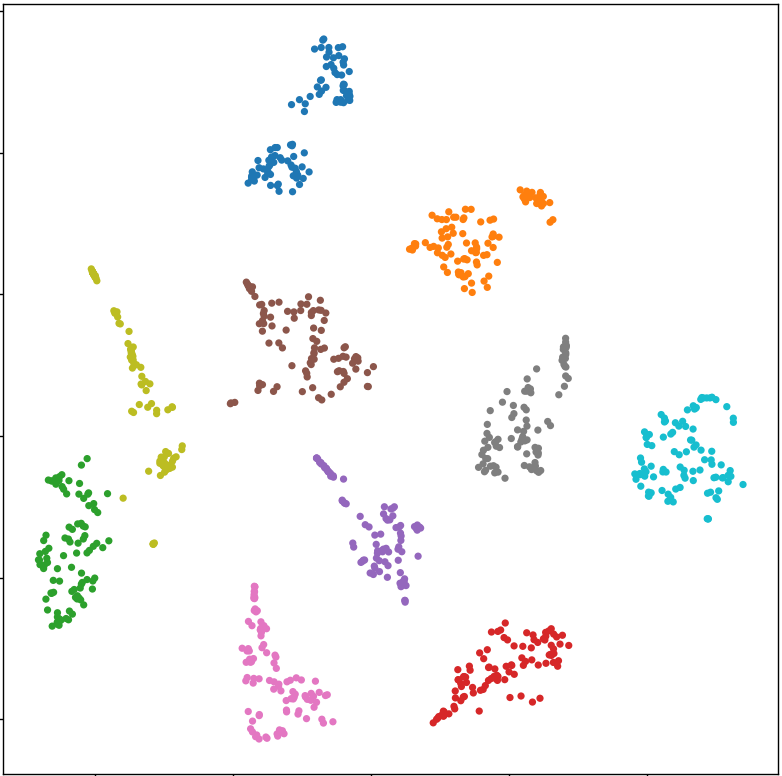
\includegraphics[width=0.32\linewidth]{simsiam_tsne.png}
        \label{simsiam_tsne}
    }
    \subfloat[]{
        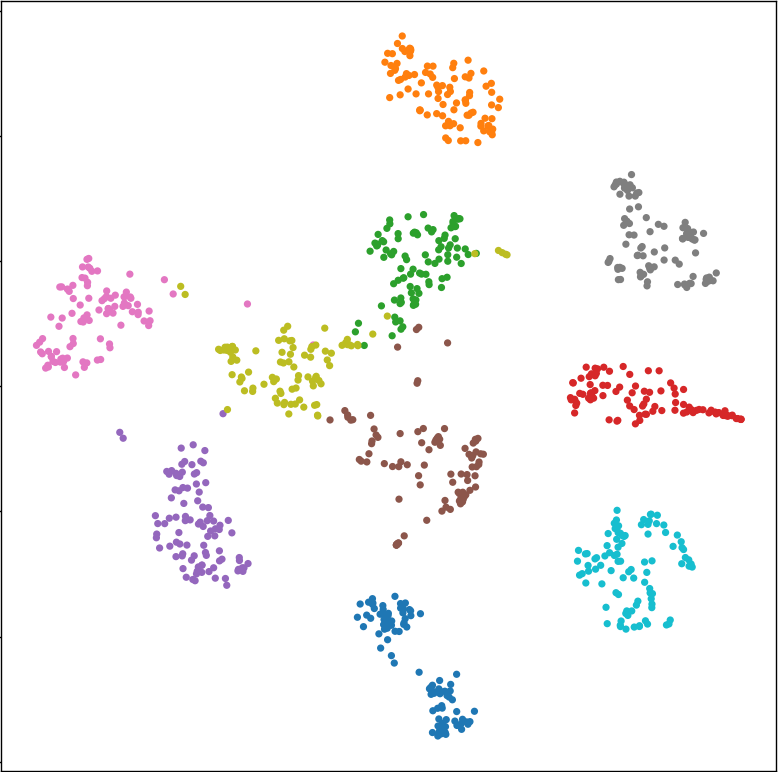
\includegraphics[width=0.32\linewidth]{cnn_tsne.png}
        \label{cnn_tsne}
    }
    \subfloat[]{
        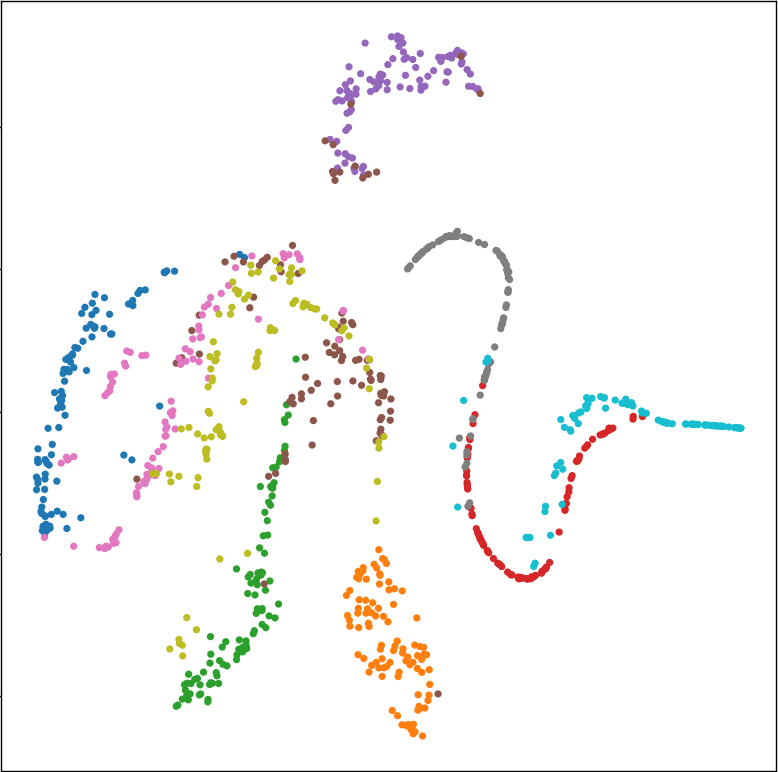
\includegraphics[width=0.32\linewidth]{svm_tsne.png}
        \label{svm_tsne}
    }
    \caption{验证集数据经特征提取的 T-SNE 可视化:(a) SimSiam 的 T-SNE 分布图;(b) CNN 的 T-SNE 分布图;(c) SVM 的 T-SNE 分布图。}
    \label{tsne_of_all}
\end{figure}

\subsection{对SimSiam网络模块的探讨}
图\ref{train_process_simsiam_discuss}展示了“使用停止梯度(Stop-Grad)”与“不使用停止梯度”的比较。架构和所有超参数保持不变,唯一的区别是是否使用停止梯度或预测器。
图\ref{train_process_simsiam_discuss:loss}显示了训练损失。不使用停止梯度时,优化器迅速找到一个退化解,并达到最小可能损失 \(-1\)。为了证明这种退化是由坍缩引起的,我们研究了 \(\ell_2\) 归一化输出 \( z / \|z\|_2 \) 的标准差(std)。如果输出坍缩到一个常数向量,则所有样本的 std 在每个通道上应该为零。这可以从图 2(中)的红色曲线中观察到。


作为对比,如果输出 \( z \) 具有零均值各向同性高斯分布,我们可以证明 \( \frac{z}{\|z\|_2} \) 的标准差为 \( \frac{1}{\sqrt{d}} \)。下证:假设 \( z \in \mathbb{R}^d \) 是一个零均值各向同性高斯分布,即 \( z \sim \mathcal{N}(0, I_d) \),其中 \( I_d \) 是 \( d \) 维单位矩阵,表示协方差矩阵为单位矩阵,意味着每个分量 \( z_i \) 独立且服从标准正态分布。我们需要证明的是,\( \frac{z}{\|z\|_2} \) 的标准差(即每个分量的标准差)为 \( \frac{1}{\sqrt{d}} \),其中 \( \|z\|_2 = \sqrt{\sum_{i=1}^{d} z_i^2} \) 是 \( z \) 的 \( L_2 \) 范数。

\textbf{证明步骤}:

\begin{enumerate}
    \item \textbf{标准化操作}:
    设 \( z = (z_1, z_2, \dots, z_d) \),则 \( z \) 的每个分量 \( z_i \) 都是独立的标准正态随机变量 \( z_i \sim \mathcal{N}(0, 1) \),并且 \( \|z\|_2 = \sqrt{\sum_{i=1}^{d} z_i^2} \) 是 \( z \) 的欧几里得范数。我们关注的是向量 \( \frac{z}{\|z\|_2} \) 的每个分量。

    \item \textbf{定义随机变量}:
    令 \( \hat{z} = \frac{z}{\|z\|_2} \),即 \( \hat{z} \) 是单位向量,表示将 \( z \) 投影到单位球面上的结果。

    \item \textbf{每个分量的分布}:
    因为 \( z \) 是各向同性高斯分布,其方向是均匀分布在单位球面上的。对于标准化后的向量 \( \hat{z} \),每个分量 \( \hat{z}_i = \frac{z_i}{\|z\|_2} \) 的分布不再是标准正态分布,而是受到范数约束的结果。

    \item \textbf{期望值和方差}:
    由于 \( z \) 是各向同性的,\( \hat{z}_i \) 的分布是对称的,所有分量 \( \hat{z}_i \) 的期望值为 0。因此,接下来我们计算 \( \hat{z}_i \) 的方差。

    对于 \( \hat{z}_i \) 的方差,我们有:
    \begin{equation}
    \text{Var}(\hat{z}_i) = \mathbb{E}[\hat{z}_i^2] - (\mathbb{E}[\hat{z}_i])^2
    \end{equation}
    由于 \( \mathbb{E}[\hat{z}_i] = 0 \),我们只需要计算 \( \mathbb{E}[\hat{z}_i^2] \)。

    \begin{equation}
    \mathbb{E}[\hat{z}_i^2] = \mathbb{E}\left[\frac{z_i^2}{\|z\|_2^2}\right] = \frac{\mathbb{E}[z_i^2]}{\mathbb{E}[\|z\|_2^2]} = \frac{1}{d}
    \end{equation}
    其中 \( \mathbb{E}[z_i^2] = 1 \)(因为 \( z_i \) 是标准正态分布),而 \( \mathbb{E}[\|z\|_2^2] = \mathbb{E}[\sum_{i=1}^{d} z_i^2] = d \),因为每个 \( z_i^2 \) 的期望为 1。

    \item \textbf{标准差}:
    由于方差 \( \text{Var}(\hat{z}_i) = \frac{1}{d} \),因此标准差是:
    \begin{equation}
    \text{std}(\hat{z}_i) = \frac{1}{\sqrt{d}}
    \end{equation}
\end{enumerate}


图\ref{train_process_simsiam_discuss:std}的红色曲线显示,使用停止梯度时,std 值接近 \( \frac{1}{\sqrt{d}} \)。这表明输出没有坍缩,而是分散在单位超球面上。
图\ref{train_process_simsiam_discuss:acc}绘制了KMeans聚类的验证准确率。KMeans聚类可以作为进展的监控工具。使用停止梯度时,监控显示出准确率稳步提高。

图\ref{train_process_simsiam_discuss}的绿色曲线显示模型在移除预测器(Predictor)后的表现,可以看出移除预测器后发生了与移除Stop-Grad类似的坍塌。事实上,如果使用对称损失(式(\ref{eq:cos_loss})),这一现象是可以预期的。现在的损失函数是
\begin{equation}
    \frac{1}{2}D(z_1, \text{stopgrad}(z_2)) + \frac{1}{2}D(z_2, \text{stopgrad}(z_1)).
\end{equation}
其梯度的方向与 $D(z_1, z_2)$ 的梯度相同,只不过幅度被缩放了 $\frac{1}{2}$。在这种情况下,使用 Stop-Grad 相当于移除 Stop-Grad 并将损失函数缩放 $\frac{1}{2}$。因此,观察到模型崩塌(图\ref{train_process_simsiam_discuss})。图\ref{tsne_simsiam_discuss}可视化了这种崩塌带来的对特征提取的影响。
表\ref{simsiam_vs_simsiamwosg_wopred}也显示了移除Stop-Grad或预测器后的巨大性能损失。
\begin{figure}
    \centering
    \subfloat[]{
        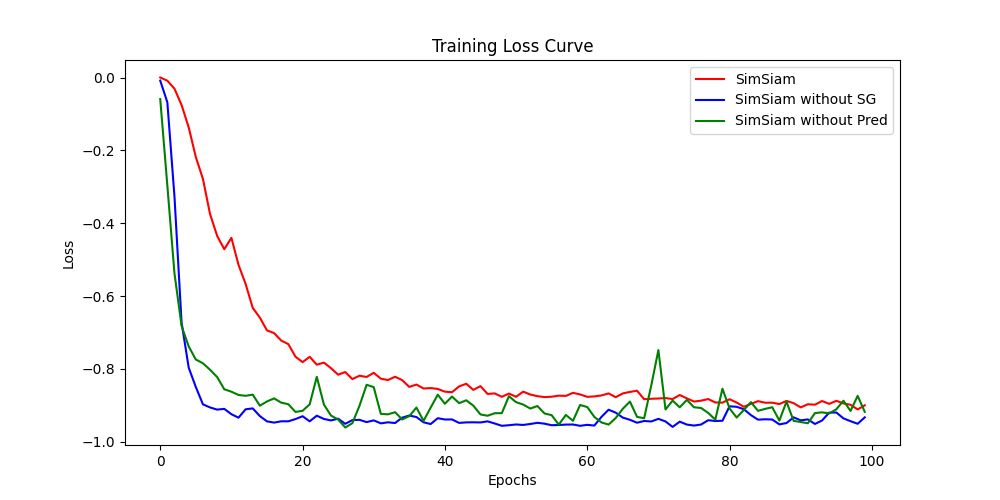
\includegraphics[width=0.45\linewidth]{loss.png}
        \label{train_process_simsiam_discuss:loss}
    }
    \subfloat[]{
        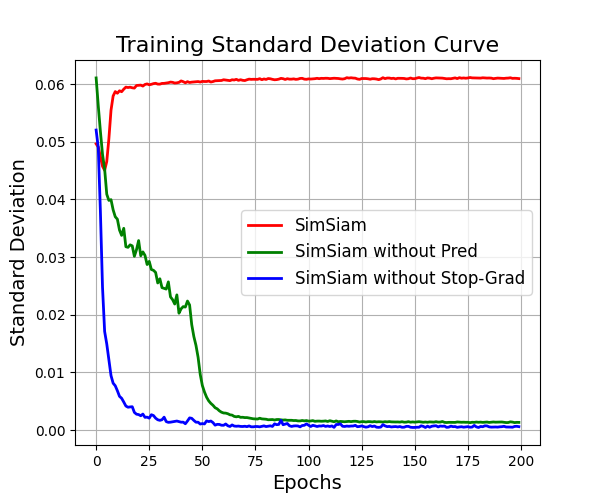
\includegraphics[width=0.45\linewidth]{std.png}
        \label{train_process_simsiam_discuss:std}
    }\\
    \subfloat[]{
        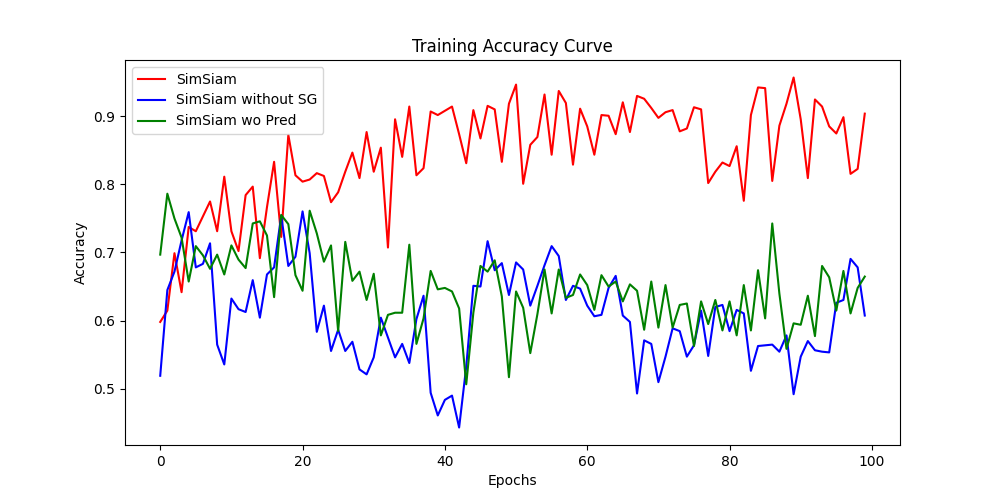
\includegraphics[width=0.45\linewidth]{acc.png}
        \label{train_process_simsiam_discuss:acc}
    }
    \caption{SimSiam,SimSiam(无Stop-Grad模块)与SimSiam(无预测器模块)的训练过程对比(a) 损失函数;(b) 提取特征的标准差;(c) K-Means聚类准确率}
    \label{train_process_simsiam_discuss}
\end{figure}

\begin{figure}
    \centering
    \subfloat[]{
        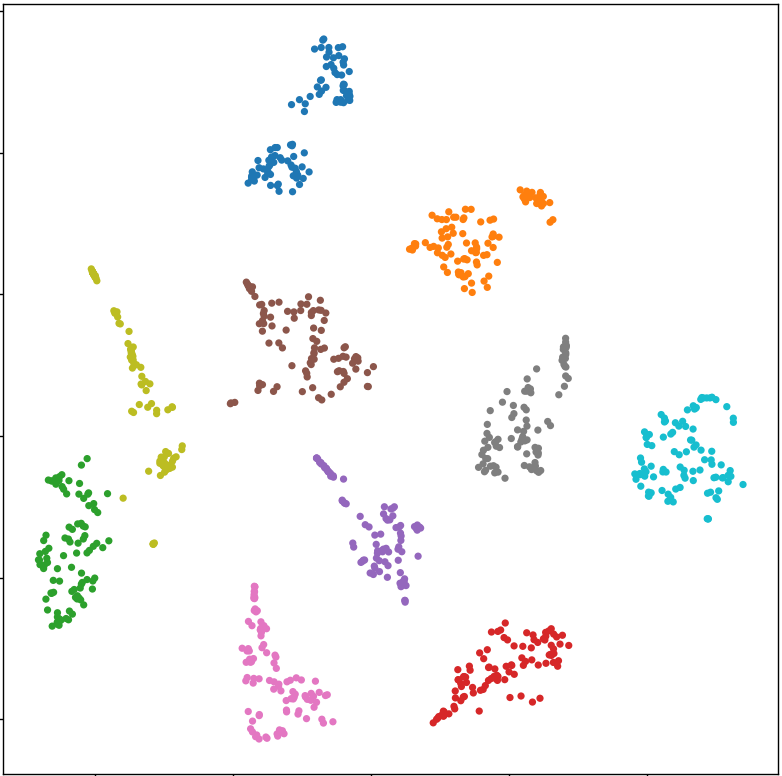
\includegraphics[width=0.3\linewidth]{simsiam_tsne.png}
        \label{tsne_simsiam_discuss:simsiam_tsne}
    }
    \subfloat[]{
        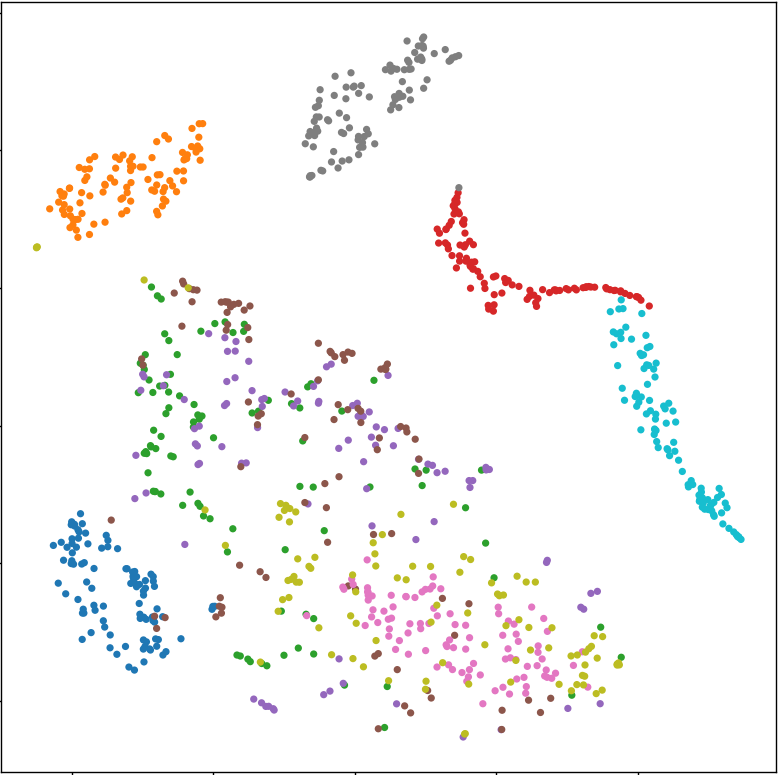
\includegraphics[width=0.3\linewidth]{simsiam_wo_stopgrad_tsne.png}
        \label{tsne_simsiam_discuss:simsiam_wo_stopgrad_tsne}
    }
    \subfloat[]{
        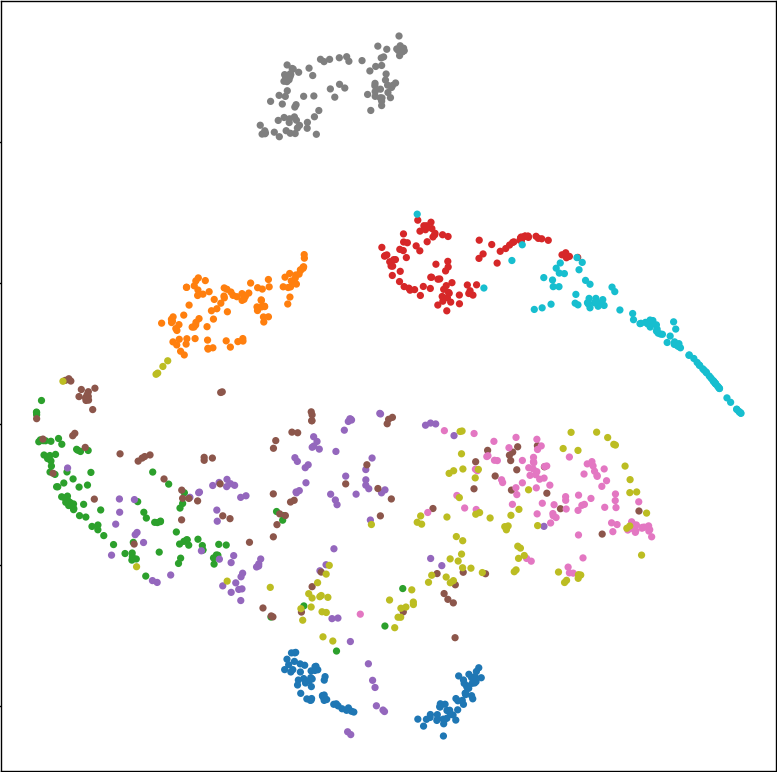
\includegraphics[width=0.3\linewidth]{simsiam_wo_pred_tsne.png}
        \label{tsne_simsiam_discuss:simsiam_wo_pred_tsne}
    }
    \caption{SimSiam,SimSiam(无Stop-Grad模块)与SimSiam(无预测器模块)的T-SNE图(a) SimSiam;(b) SimSiam without Stop-Grad;(c) SimSiam without Predictor}
    \label{tsne_simsiam_discuss}
\end{figure}

\begin{table}[h]
    \caption{SimSiam、SimSiamw/o SG 与 SimSiamw/o Pred 在不同 $\beta$ 值下的准确率}
    \centering
    \begin{tabular}{cccc}
    \toprule
    不平衡因子$\beta$  & SimSiam & SimSiamw/o SG & SimSiamw/o Pred \\
    \midrule
    1   & 0.9515  & 0.5338  & 0.5217 \\
    2   & 0.9517  & 0.5025  & 0.5575 \\
    5   & 0.9315  & 0.4496  & 0.4952 \\
    10  & 0.9402  & 0.4919  & 0.4604 \\
    50  & 0.9131  & 0.3579  & 0.3892 \\
    100 & 0.8450  & 0.3412  & 0.3704 \\
    \midrule
    平均值 & 0.9222  & 0.4462  & 0.4657 \\
    \bottomrule
    \end{tabular}
    \label{simsiam_vs_simsiamwosg_wopred}
\end{table}


\subsection{对数据增强模块的探讨}
在\ref{sec:CMA-ES_result}小节,我们在限定范围内求得了各个数据增强子策略的最优参数解,并在之后的实验中取得了良好的结果。本节讨论表\ref{CMA-ES_solution}中的8个数据增强子策略对模型性能的影响。图\ref{train_process_da_discuss}显示了移除单个子策略后模型训练过程中的损失函数及特征标准差。
\begin{figure}
    \centering
    \subfloat[]{
        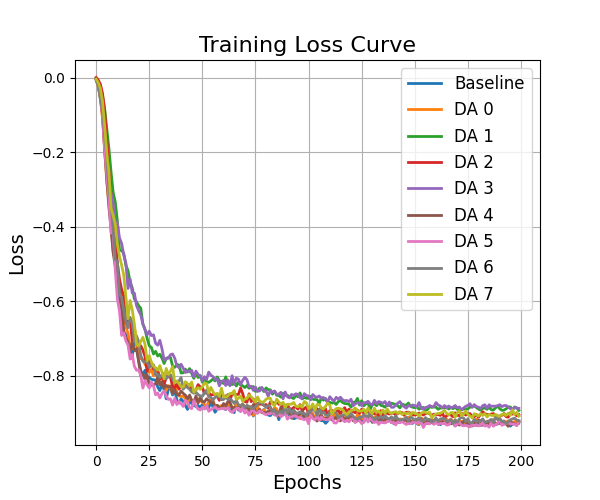
\includegraphics[width=0.45\linewidth]{loss_da.png}
        \label{train_process_da_discuss:loss}
    }
    \subfloat[]{
        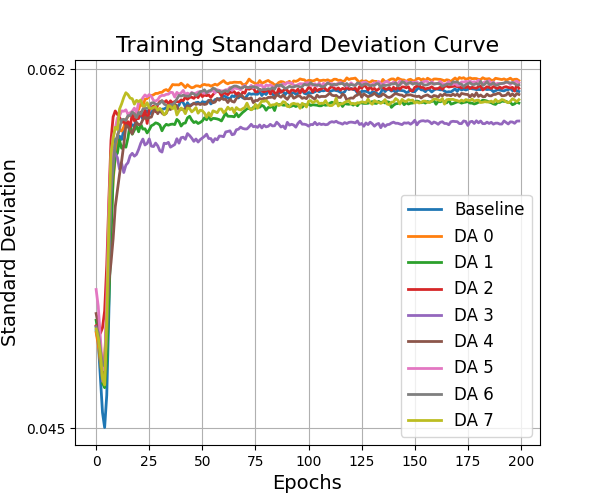
\includegraphics[width=0.45\linewidth]{std_da.png}
        \label{train_process_da_discuss:std}
    }
    \caption{移除不同数据增强子策略的训练过程对比(a) 损失函数;(b) 提取特征的标准差;}
    \label{train_process_da_discuss}
\end{figure}

\begin{table}[h]
    \caption{移除不同数据增强子策略在不同 $\beta$ 值下的准确率}
    \centering
    \begin{tabular}{ccccccccc}
    \toprule
    不平衡因子$\beta$  & DA0 & DA1 & DA2 & DA3 & DA4 & DA5 & DA6 & DA7 \\
    \midrule
    1   & 0.9279  & 0.9127 & 0.9254 & 0.9204 & 0.9106 & 0.9298 & 0.9394 & 0.9338  \\
    2   & 0.9219  & 0.9121 & 0.9223 & 0.9275 & 0.9183 & 0.9333 & 0.9427 & 0.9456  \\
    5   & 0.9246  & 0.8969 & 0.8940 & 0.9217 & 0.8810 & 0.9088 & 0.9117 & 0.9310  \\
    10  & 0.9258  & 0.9348 & 0.8944 & 0.9298 & 0.8792 & 0.9358 & 0.9333 & 0.9442  \\
    50  & 0.8563  & 0.8379 & 0.8221 & 0.8467 & 0.7490 & 0.8165 & 0.8573 & 0.8387  \\
    100 & 0.7935  & 0.8169 & 0.7356 & 0.7194 & 0.7119 & 0.7912 & 0.8333 & 0.7869  \\
    \midrule
    平均值 & 0.8836  & 0.8852 & 0.8656 & 0.8776 & 0.8417 & 0.8859 & 0.9029 & 0.8967 \\
    \midrule
    相比Baseline & -0.0386 & -0.0370 & -0.0566 & -0.0446 & -0.0805 & -0.0363 & -0.0193 & -0.0255 \\
    \bottomrule
    \end{tabular}
    \label{checkpoint_results_with_avg}
\end{table}



\section{本章小结}

\chapter{基于半监督学习和分类面调整算法的微调方法研究}
在上一章中,我们展示了自监督学习范式中的二阶段式训练(如图\ref{self_supervise_procedure}所示)在故障诊断任务中的长尾学习场景下,显著提升了模型性能。然而,在微调阶段,样本分布的不平衡仍会影响模型,导致分类器的决策面发生偏移。如图\ref{decision_edge_bias}所示,决策面会朝尾部类的空间偏移,导致头部类在特征空间中占据更大的体积,从而降低了模型对尾部类的分类准确率。在本章节中,我们将深入探讨半监督学习与决策面调整算法,旨在减轻长尾分布对微调阶段决策面偏移的影响,从而提高尾部类的识别能力。

\begin{figure}[h]
    \centering
    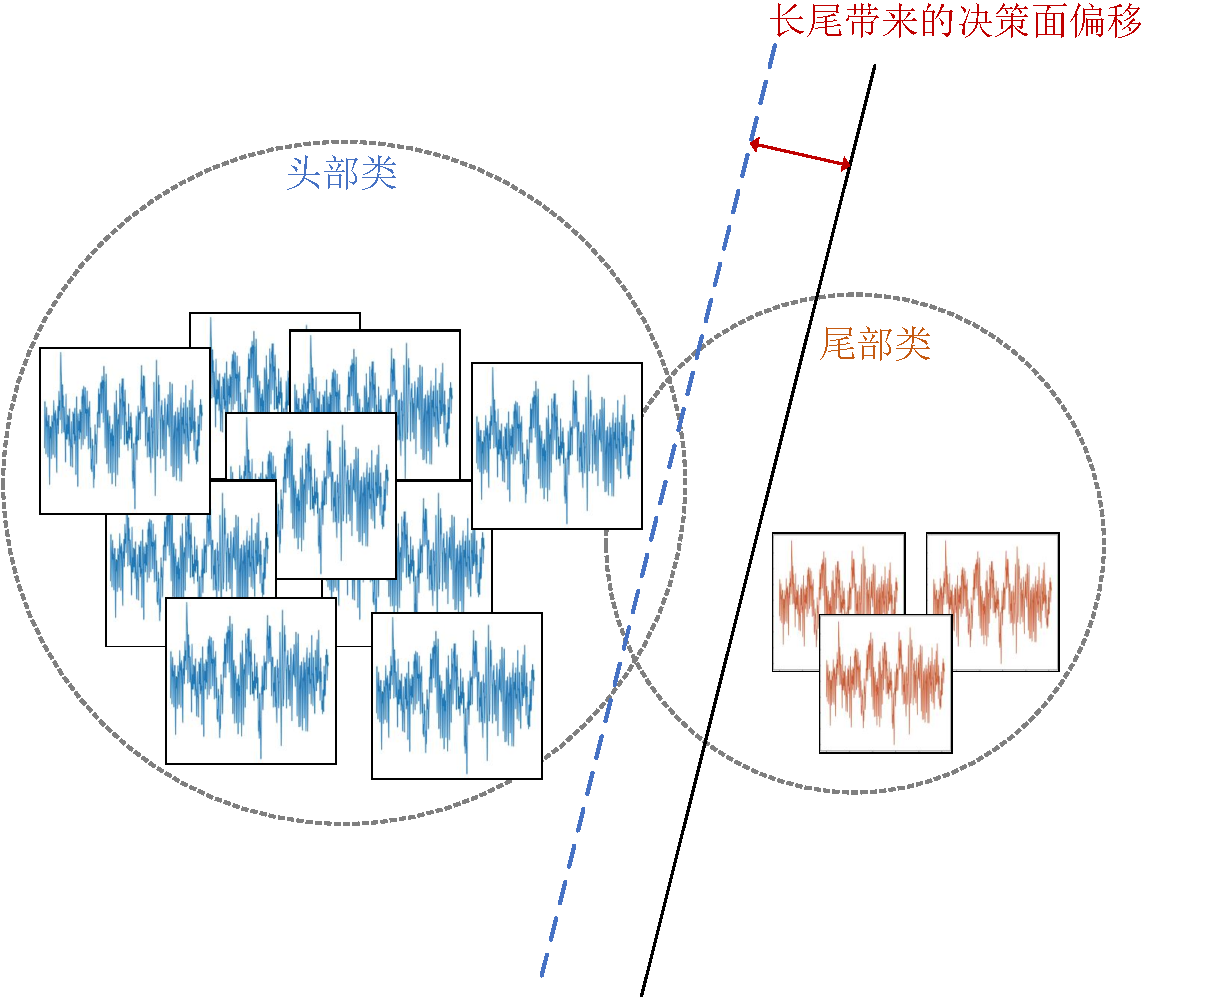
\includegraphics[width=12cm]{decision_edge_bias.pdf}
    \caption{由长尾分布带来的决策面偏移示意图}
    \label{decision_edge_bias}
\end{figure}

\section{模型架构}
\subsection{半监督学习模型架构}
本研究提出了一种结合半监督学习与决策边界调整的框架,以有效解决长尾分布和样本不平衡问题。受到文献\cite{yang2020rethinking,wang2023margin}的启发,研究借鉴了半监督学习的经典流程(如图\ref{semi_supervise_procedure}所示)。该流程分为两个阶段:

在第一阶段,使用原始的不平衡标记数据集 $\mathcal{D}_{L}$ 训练一个初步分类器 $f_{\hat{\theta}}$。随后,在第二阶段,利用该分类器对未标记数据集 $\mathcal{D}_{U}$ 进行推断并生成伪标签 $\hat{y}$。伪标签数据与标记数据结合,通过最小化以下损失函数优化模型:
\begin{equation} 
    \mathcal{L}(\mathcal{D}_{L},\theta) + \omega \mathcal{L}(\mathcal{D}_{U},\theta), 
\end{equation}
其中,$\omega$ 为未标记数据的损失权重,$\mathcal{L}(\mathcal{D}_{L},\theta)$ 和 $\mathcal{L}(\mathcal{D}_{U},\theta)$ 分别代表基于标记数据和伪标签数据的损失项。通过整合这两部分损失,最终得到优化后的分类器 $f_{\hat{\theta_f}}$,以更好地建模数据分布,尤其是尾部类别(少数类别)。该过程通过充分利用未标记数据 $\mathcal{D}_{U}$,提升模型对少数类别的分类能力,从而显著优化其决策边界。

\begin{figure}[h]
    \centering
    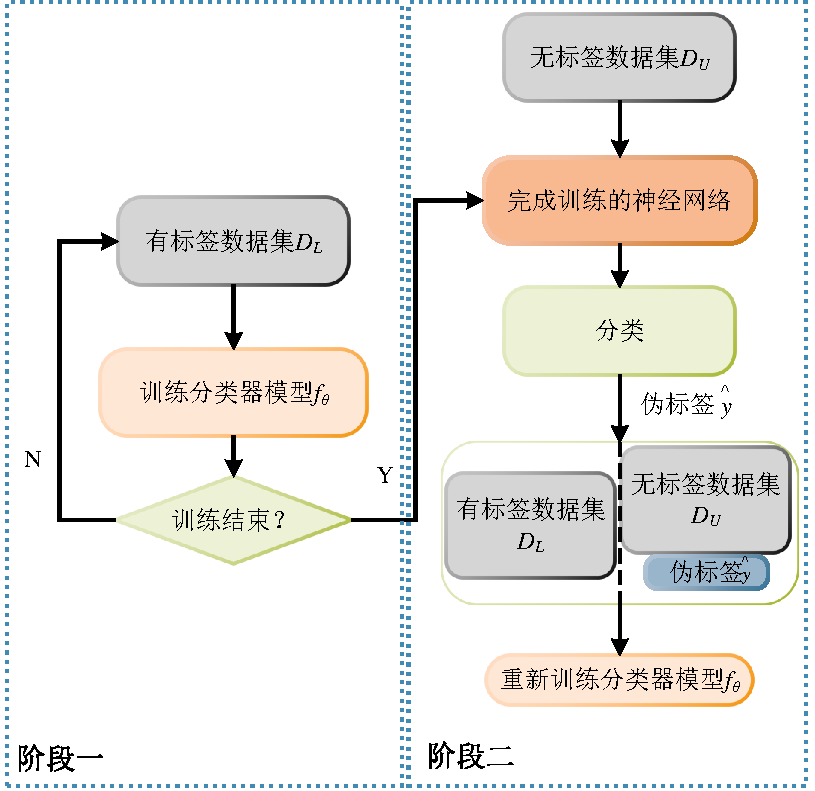
\includegraphics[width=12cm]{semi_supervise_procedure.pdf}
    \caption{半监督学习流程图}
    \label{semi_supervise_procedure}
\end{figure}

与此同时,在处理长尾分布和样本不平衡问题时,决策面调整方法(MARC)提供了一种有效的方式来改善分类器的性能,特别是在少数类别(尾部类别)上。文献\cite{wang2023margin}介绍的决策面调整算法通过引入边界校准方法,调整分类器的决策面,使其更加均衡地处理各个类别的数据。

MARC算法包括两个关键参数:$\omega$ 和 $\beta$,其中 $\omega$ 是用于调整输出的尺度因子,而 $\beta$ 则是用于调整输出的偏置项。这两个参数通过最小化损失函数来进行优化,从而获得适合当前任务的最优决策面。算法的具体实现步骤参考表\ref{alg:marc}。在MARC伪代码中,$\omega$ 和 $\beta$ 是通过 \verb|torch.nn.Parameter| 初始化为可训练的参数,它们分别表示边界的缩放因子和偏置项。使用 \verb|torch.no_grad()| 关键字来避免计算梯度,确保在前向传播时不会影响到梯度计算。接下来,代码通过计算网络的权重范数以及模型在给定输入 $x$ 上的输出结果,来调整输出的决策面,生成校准后的输出 $\text{logit\_after}$。在实际应用中,MARC 算法有助于减小尾部类别的分类误差,尤其是在样本不平衡的情况下,通过有效地调整决策边界来改善模型的泛化能力和分类精度。

\begin{table}[h]
    \centering
    \begin{tabular}{@{}l@{}} % 使用 @{} 去掉默认的左右边距,l 表示左对齐
    \toprule
    \multicolumn{1}{@{}l@{}}{\textbf{MARC伪代码(用Pytorch描述)}} \\ % 左对齐文本
    \midrule
    \begin{lstlisting}[basicstyle=\ttfamily,frame=none]
1: 初始化边界校准方法:
    omega = torch.nn.Parameter(torch.ones(1, num_classes))
    beta = torch.nn.Parameter(torch.zeros(1, num_classes))

2: 输入:训练数据 x,标准的预训练神经网络模型。

3: with torch.no_grad():
4:     w_norm = torch.norm(model.fc.weight, dim=1)
5:     logit_before = model(x)
6:     logit_after = omega * logit_before + beta * w_norm
7: 计算损失并更新参数 omega 和 beta。
    \end{lstlisting} \\
    \hline
    \end{tabular}
    \caption{MARC 算法的实现步骤}
    \label{alg:marc}
\end{table}

基于上述半监督学习和 MARC 决策边界调整算法,本研究改进了上一章的SimSiam架构,提出了一种结合两者的 SimSiam 模型架构,称为 \textbf{基于半监督学习和 MARC 微调的 SimSiam 模型}。该模型通过三阶段的逐步优化,旨在解决长尾分布和样本不平衡问题,并显著提升分类器在尾部类别上的性能。其具体架构流程如图 \ref{semi_marc_simsiam} 所示。
该模型架构包括以下三个阶段:

\begin{enumerate}
    \item \textbf{阶段一(自监督学习)}:  
    在第一阶段,基于 SimSiam 架构对模型进行预训练。具体而言,利用大量无标签样本和少量有标签的长尾样本,训练一个性能较优的特征提取网络和初步分类器。SimSiam 的自监督特性能够在数据量受限的情况下充分挖掘数据的潜在分布信息,为后续的半监督学习提供高质量的特征表示。

    \item \textbf{阶段二(半监督学习)}:  
    在第二阶段,基于阶段一训练得到的 SimSiam 模型,使用其生成无标签样本的伪标签(Pseudo Labels),将伪标签视为无标签数据的“真实标签”。随后,将补充有伪标签的无标签数据与原始有标签数据集相结合,通过最小化标记数据和伪标签数据的损失函数,重新优化分类器的全连接层参数。这一阶段的目标是进一步提高模型的泛化能力,尤其是在尾部类别上的表现。

    \item \textbf{阶段三(MARC 决策边界调整)}:  
    在第三阶段,利用经过半监督学习优化后的分类器及其输出的 logits,对决策边界进行微调。具体而言,通过训练两个向量参数 $\omega$ 和 $\beta$,分别控制分类器输出的尺度因子和偏置项,调整分类器的决策面,以提升模型在尾部类别上的分类准确率。MARC 的引入有效平衡了模型在头部类别和尾部类别上的性能差异。
\end{enumerate}

\begin{figure}[h]
    \centering
    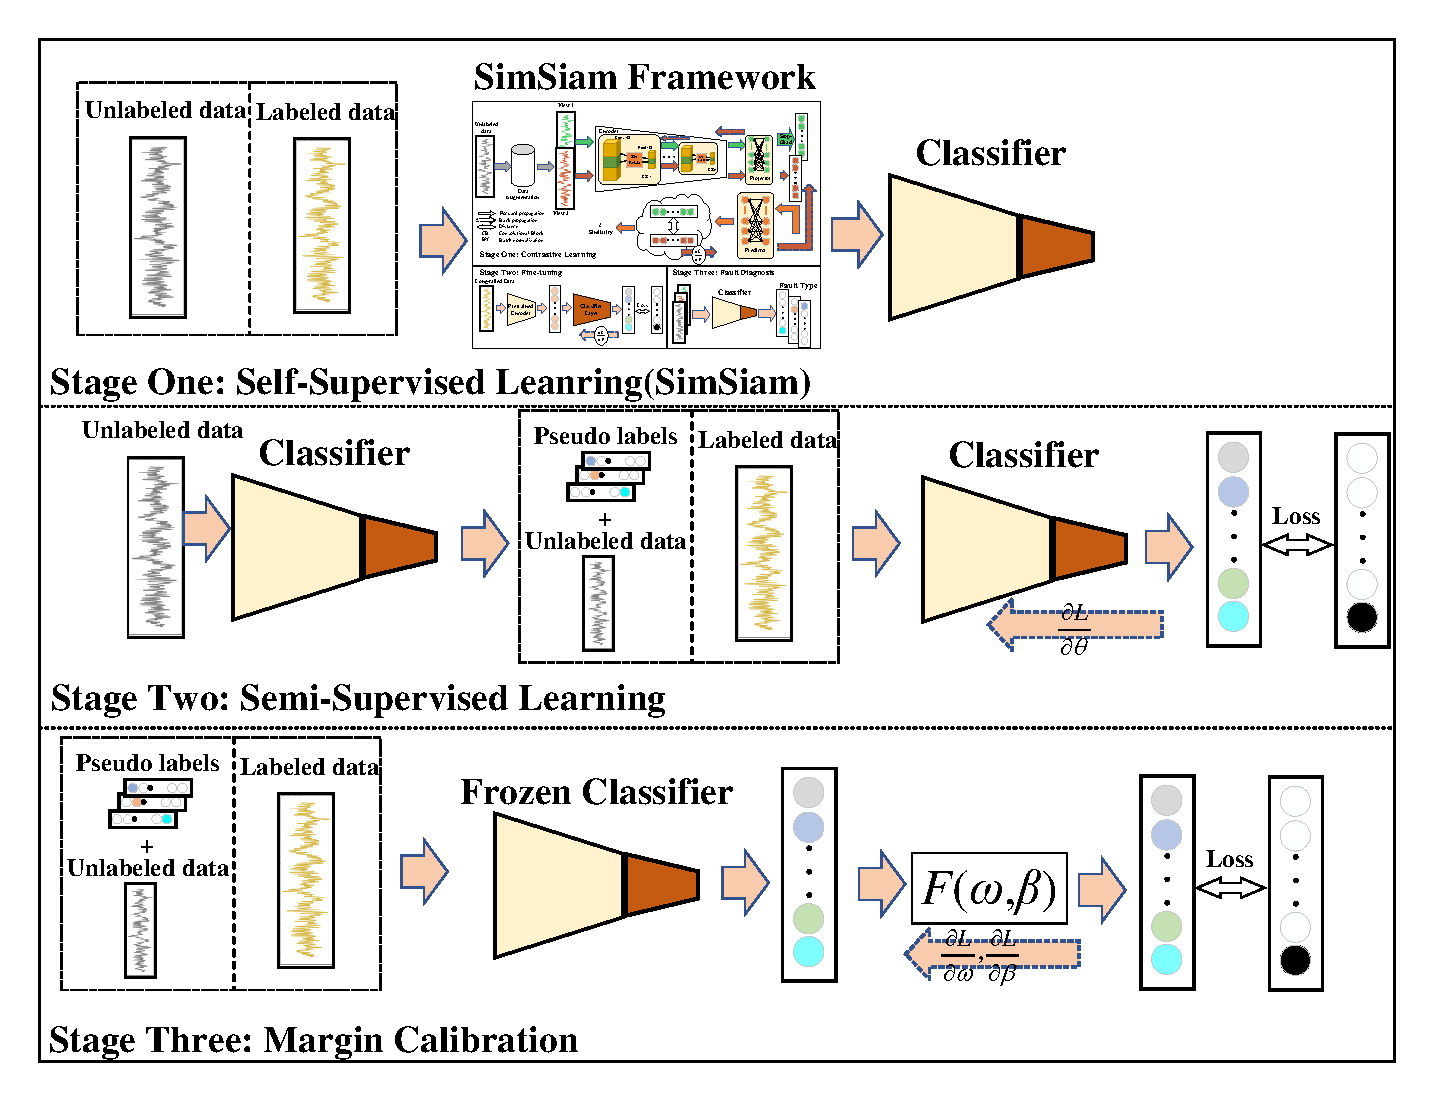
\includegraphics[width=12cm]{semi_marc_simsiam.pdf}
    \caption{基于半监督学习和 MARC 微调的 SimSiam 模型流程框图}
    \label{semi_marc_simsiam}
\end{figure}

整体流程通过结合 SimSiam 的特征提取能力、半监督学习对伪标签的利用,以及 MARC 算法对决策边界的微调,形成了一个多阶段优化框架。该方法在处理长尾分布和样本不平衡问题时,展现出显著的优势,尤其是在提高尾部类别分类准确率方面效果显著。

\section{实验与分析}
采用CWRU数据集,数据集构造方法与\ref{simsiam_cwru_results}节相同。一阶段训练150个周期,二阶段重新训练150个周期。在不同不平衡因子下的准确率结果如表\ref{simsiam_semi_results}所示。

\begin{table}[h]
    \caption{SimSiam 与 Semi 在不同 $\beta$ 值下的准确率}
    \centering
    \begin{tabular}{cccccc}
    \toprule
    不平衡因子$\beta$  & SimSiam & Semi & Marc & Semi\_Marc \\
    \midrule
    1   & 0.9515  & 0.9813 & 0.94896 & 0.9781 \\
    2   & 0.9517  & 0.9656 & 0.95917 & 0.9698 \\
    5   & 0.9315  & 0.9406 & 0.94021 & 0.9615 \\
    10  & 0.9402  & 0.9573 & 0.9575  & 0.9615 \\
    50  & 0.9131  & 0.9344 & 0.91687 & 0.9271 \\
    100 & 0.8450  & 0.9031 & 0.87896 & 0.9406 \\
    \bottomrule
    \end{tabular}
    \label{simsiam_semi_results}
\end{table}


\chapter{其他长尾学习方法分析(CB LOSS等)}

\section{}


\section{本章小结}


\chapter{全文总结与展望}

\section{全文总结}

\section{后续工作展望}

\thesisacknowledgement
在攻读博士学位期间,首先衷心感谢我的导师XXX教授

\thesisappendix

\chapter{中心极限定理的证明}

\section{高斯分布和伯努利实验}


% Uncomment to list all the entries of the database.
% \nocite{*}

\thesisbibliography{reference}

%
% Uncomment following codes to load bibliography database with native
% \bibliography command.
%
% \nocite{*}
% \bibliographystyle{thesis-uestc}
% \bibliography{reference}
%

\thesisaccomplish{publications}

\end{document}
